\documentclass[compsoc,conference,a4paper,10pt,times]{IEEEtran}
\IEEEoverridecommandlockouts
% The preceding line is only needed to identify funding in the first footnote. If that is unneeded, please comment it out.
\usepackage{cite}
\usepackage{amsmath,amssymb,amsfonts}
\usepackage{algorithmic}
\usepackage{graphicx}
\usepackage{textcomp}
\usepackage{bmpsize}
\usepackage{xcolor}
\usepackage{lipsum}
\usepackage[colorlinks=true,urlcolor=black]{hyperref}
\def\BibTeX{{\rm B\kern-.05em{\sc i\kern-.025em b}\kern-.08em
    T\kern-.1667em\lower.7ex\hbox{E}\kern-.125emX}}

\newcommand{\garrison}[1]{\textcolor{blue}{Garrison: #1}}
\usepackage{soul}
\usepackage{multirow}
\usepackage{tikz}
\usepackage{epsfig} 
\usepackage{xfrac}
\usepackage{filecontents}
\usepackage{csquotes}
\usepackage{footnote}
\makesavenoteenv{tabular}
\makesavenoteenv{table}
\usepackage{pifont}
\usepackage{pbox}
\usepackage{cancel}
\newtheorem{theorem}{Theorem}
\newtheorem{corollary}{Corollary}[theorem]
\newtheorem{lemma}[theorem]{Lemma}
\newtheorem{remark}[theorem]{Remark}
%\theoremstyle{definition}
\newtheorem{definition}{Definition}[section]
\newtheorem{proof}[theorem]{Proof}
\usepackage{subcaption}

\begin{document}

\title{RLSA-PFL: Robust Lightweight Secure Aggregation with Model Inconsistency Detection in Privacy-Preserving Federated Learning}

\author{\IEEEauthorblockN{Nazatul H. Sultan}
\IEEEauthorblockA{CSIRO's Data61, Australia}
\and
\IEEEauthorblockN{Yan Bo}
\IEEEauthorblockA{CSIRO's Data61, Australia}
\and
\IEEEauthorblockN{Yansong Gao}
\IEEEauthorblockA{CSIRO's Data61, Australia}
\and
\IEEEauthorblockN{Seyit Camtepe}
\IEEEauthorblockA{CSIRO's Data61, Australia}

\and
\IEEEauthorblockN{Arash Mahboubi}
\IEEEauthorblockA{CSU, Australia}

\and
\IEEEauthorblockN{Hang Thanh Bui}
\IEEEauthorblockA{CSU, Australia}

\and
\IEEEauthorblockN{Aufeef Chauhan}
\IEEEauthorblockA{The University of Adelaide, Australia}

\and
\IEEEauthorblockN{Hamed Aboutorab}
\IEEEauthorblockA{CSU, Australia}
\and
\IEEEauthorblockN{Michael Bewong}
\IEEEauthorblockA{CSU, Australia}
\and
\IEEEauthorblockN{Dineshkumar Singh}
\IEEEauthorblockA{TCS, Australia}
\and
\IEEEauthorblockN{Praveen Gauravaram}
\IEEEauthorblockA{TCS, Australia}
\and
\IEEEauthorblockN{Rafiqul Islam}
\IEEEauthorblockA{CSU, Australia}

\and
\IEEEauthorblockN{Sharif Abuadbba}
\IEEEauthorblockA{CSIRO's Data61, Australia}

}

\maketitle

\begin{abstract}
Federated Learning (FL) allows users to collaboratively train a global machine learning model by sharing local model only, without exposing their private data to a central server. This distributed learning is particularly appealing in scenarios where data privacy is crucial, and it has garnered substantial attention from both industry and academia. However, studies have revealed privacy vulnerabilities in FL, where adversaries can potentially infer sensitive information from the shared model parameters. In this paper, we present an efficient masking-based secure aggregation scheme utilizing lightweight cryptographic primitives to mitigate privacy risks. Our scheme offers several advantages over existing methods. First, it requires only a single setup phase for the entire FL training session, significantly reducing communication overhead. Second, it minimizes user-side overhead by eliminating the need for user-to-user interactions, utilizing an intermediate server layer and a lightweight key negotiation method. Third, the scheme is highly resilient to user dropouts, and the users can join at any FL round. Fourth, it can detect and defend against malicious server activities, including recently discovered model inconsistency attacks. Finally, our scheme ensures security in both semi-honest and malicious settings. We provide security analysis to formally prove the robustness of our approach. Furthermore, we implemented an end-to-end prototype of our scheme\footnote{The fully foundational end-to-end source code will be released upon publication.}. We conducted comprehensive experiments and comparisons, which show that it outperforms existing solutions in terms of communication and computation overhead, functionality, and security. 
\end{abstract}

\begin{IEEEkeywords}
Federated Learning, Machine Learning, Privacy, Secure Aggregation, User Dropouts, Model Inconsistency Attack.
\end{IEEEkeywords}

\section{Introduction}
\label{intro}
Federated Learning (FL) is a distributed machine learning (ML) approach designed to enhance user privacy during the model training process. Instead of sending user data to a central server, FL only shares local model updates after training happens on the users' devices. The central server then combines these updates to create a global model without ever accessing the actual data \cite{Liu2022}. This distributed system reduces the chance of sensitive information being exposed, improving both privacy and security. FL is already being used in areas like healthcare \cite{Antunes2022}, telecommunications \cite{Niknam2020}, the Internet of Things (IoT) \cite{Khan2021}, and smart cities \cite{Pang2024}.
\par 
However, FL on its own cannot fully eliminate privacy risks. Zhu \emph{et al.} \cite{Zhu2019} showed that attackers, including the central server, could still reconstruct users' local datasets by exploiting the gradients shared during model updates. Similar risks have been found in other studies \cite{Geiping2020, zhou2023ppa, Jeon2024}, where researchers pointed out that sharing gradients with the central server could reveal sensitive user data. As a result, additional security measures are needed to fully protect privacy in FL. One popular solution is combining FL with privacy-preserving techniques like differential privacy (DP) \cite{Liu2022}. However, DP comes with a trade-off: the stronger the privacy protection, the more it deteriorates the utility of the global model \cite{Chen2024}.
\par 
Secure aggregation is an alternative promising privacy-preserving technique that has gained significant attention for its advantages over DP, such as maintaining accuracy, simplicity in implementation, and avoiding trade-offs in utility \cite{Yin2021}. In this method, users cryptographically hide their local model updates before sharing them with the central server. The server then aggregates these hidden updates without being able to view the individual contributions. This ensures that no single party, including the central server, can reconstruct individual model parameters while still obtaining an accurate aggregated global model. Secure aggregation effectively mitigates privacy risks like gradient leakage, which could otherwise expose sensitive data \cite{Liu2022}.
\par 
In general, secure aggregation relies on cryptographic primitives such as homomorphic encryption (HE), secure multi-party computation (SMC), and masking-based techniques \cite{Liu2022}. Among these, masking-based secure aggregation is often considered more practical than the others due to its relatively lower computational and communication costs \cite{Yin2021}. Several masking-based secure aggregation protocols have been proposed in recent years, including foundational techniques like the BBGLR protocol by Bonawitz \emph{et al.} in \cite{Bonawitz2017}. BBGLR employs a cryptographic masking technique that allows users to securely mask their local model updates before aggregation, ensuring that the central server cannot reconstruct individual updates while still generating the global model. Building on this work, various protocols (e.g., \cite{Bell2020, Eltaras2023, Fereidooni2021, Guo2021, Liu2023, Xu2020}) have introduced improvements to enhance security and reduce computational or communication overhead, optimizing FL for diverse real-world applications.
\par 
 However, the BBGLR protocol and its variants have some limitations. One issue is the computational overhead for users due to the user-to-user secret-sharing mechanism. Users need to generate shared keys with their neighbors and perform cryptographic operations like additive secret sharing, which increases computational complexity, especially for devices with limited resources. Another challenge is the communication overhead, as users must exchange secret shares with neighbors in every round of training, requiring a fresh setup each time \cite{Ma2023}. This imposes a significant communication burden, particularly in large-scale FL systems. Since secret sharing is repeated in each round, the scalability becomes a concern, as the overhead grows with both the number of participants and the training rounds. This problem is even more pronounced in scenarios with many users and rounds, as noted in \cite{Ma2023}. %Further details on the related works and their limitations will be provided in Section \ref{sec:related-work}. 
\par 
Moreover, a recent study by Pasquini \emph{et al.} \cite{Pasquini2022} demonstrated that the BBGLR protocol and it's variants are vulnerable to a new type of attack known as \emph{model inconsistency}, particularly when the central server is malicious. This issue also affects other FL systems using secure aggregation techniques like SMC and HE. The key idea behind this attack is that the server controls the updates used in secure aggregation. A malicious server can manipulate these updates to make the final results reveal information about one or more targeted users, undermining the protection secure aggregation is supposed to offer when the central server is compromised.

\subsection{Our Contribution}
\label{sec:contribution}
In this paper, we propose a lightweight masking-based secure aggregation scheme for FL that can also detect model inconsistency attacks caused by a malicious server. Our scheme is lightweight in the sense that it only requires one setup phase for entire rounds of FL training, unlike the BBGLR protocol, which requires repeated setups. This reduces both the communication and computational load on users. Additionally, our scheme utilizes a lightweight additive secret-sharing mechanism with key negation for masking, which is more computationally efficient than the BBGLR protocol's use of the comparatively expensive \emph{Shamir's Secret Sharing}. 
\par 
Further, our scheme uses a small number of intermediate servers instead of having users interact with each other. These servers collect masked models from the users and assist the central server, referred to as the Aggregator, in handling user dropouts. Adding this middle layer offers two key benefits. First, it removes the need for user-to-user interaction, which would otherwise impose an unacceptable burden on resource-limited users \cite{Liu2023}. Second, intermediate servers are generally more trusted and reliable than other users, as they could be service providers or entities with higher reputations, resources, and trustworthiness. For example, in real-world deployments, companies like Amazon Web Services (AWS), and Microsoft Azure could act as intermediate servers, providing the necessary infrastructure to handle aggregation, ensuring trustworthiness, and maintaining high performance for scalability. 
\par 
 
Our scheme also includes an efficient global model consistency detection mechanism, though it comes with some extra communication costs. We use a message authentication code (MAC) to check for any inconsistencies in the global model received by each user. The intermediate servers play a role in receiving the MACed global models. As long as at least one intermediate server and two users are trustworthy, our scheme can successfully detect model inconsistency attacks.
\par 
In summary, our scheme offers the following contributions: \begin{itemize} 
\item We propose a novel secure aggregation method using a lightweight additive secret-sharing mechanism with key negation. It is highly resilient to user dropouts without requiring users to interact with each other or go through multiple complicated setup phases.
\item Our scheme introduces an efficient mechanism to detect model inconsistency attacks, with minimal communication costs.
\item We provide formal security proofs demonstrating our scheme's robustness against both semi-honest and malicious adversaries. 
\item We thoroughly analyze and compare our scheme with closely related works, showing superior performance across computation, communication, functionality, and security. 
\item We implemented our scheme in an end-to-end manner and provided comprehensive experimental results, demonstrating its practicality and effectiveness. %We will make our codes available upon acceptance availability and reproducibilty. %\hl{Our code is available at} \url{******}.
\end{itemize}

The organization of this paper is as follows: Section \ref{sec:related-work} provides a brief overview of related works in privacy-preserving aggregation techniques in FL. The cryptographic primitives used in our scheme are presented in Section \ref{sec:preli}. Section \ref{sec:architecture-threat-model} outlines the system architecture, threat model, assumptions, and goals of our scheme. Section \ref{sec:our_scheme} details our proposed scheme. The security analysis and performance evaluation are covered in Sections \ref{sec:sec_analysis} and Section \ref{sec:performance_eval}, respectively. Finally, the paper concludes in Section \ref{sec:conclusion}.

\begin{table*}[!t]
\centering
\caption{Comparison of Computation Complexity, Communication Overhead, Security, and Functionality between Our Scheme and Notable Masking-Based Secure Aggregation Schemes.}
\label{table:fun-com-commu-comparison}
\tiny
\begin{tabular}{|l|p{.6cm}p{.5cm}p{1.2cm}|llp{1cm}|p{.6cm}|p{.6cm}|p{1cm}|p{.6cm}|p{.8cm}|}
\hline
\multirow{2}{*}{Schemes} & \multicolumn{3}{c|}{Computation Overhead} & \multicolumn{3}{c|}{Communication Overhead} & Threat Model & Dropout & Communication Round & No. of Setup Phase & Model Incon. Attack Detection\\ \cline{2-7} 
 & \multicolumn{1}{l|}{User} & \multicolumn{1}{l|}{Intermediate Server} & Aggregator & \multicolumn{1}{l|}{User} & \multicolumn{1}{l|}{Intermediate Server} & Aggregator & & & &  & \\ \hline
   SecAgg \cite{Bonawitz2017} &\multicolumn{1}{p{1.1cm}|}{$\mathcal{O}(m^2+ m\cdot |v|)$}&\multicolumn{1}{l|}{NA}&\multicolumn{1}{p{1.1cm}|}{$\mathcal{O}(m^2+ m\cdot |v|)$}&\multicolumn{1}{p{1cm}|}{$\mathcal{O}(m+ |v|)$}&\multicolumn{1}{l|}{NA}&\multicolumn{1}{p{1.1cm}|}{$\mathcal{O}(m^2+ m\cdot |v|)$}& Malicious & $\frac{m}{3}$ & $4$ & $|i|$ & No\\\hline
 SecAgg+ \cite{Bell2020} & \multicolumn{1}{p{1.1cm}|}{$\mathcal{O}(|v|\cdot\log m+ \log m)$} & \multicolumn{1}{l|}{NA} & $\mathcal{O}(m\cdot |v|+ m\log m)$ & \multicolumn{1}{p{1.1cm}|}{$\mathcal{O}(|v|+ \log m)$} & \multicolumn{1}{l|}{NA} & $\mathcal{O}(m\cdot |v|+ m\log m)$ & Malicious& $\sigma\cdot m$ & $3$ &$|i|$ & No\\ \hline
%TurboAgg \cite{So2021} & \multicolumn{1}{l|}{$\mathcal{O}(|v|\cdot \log m \cdot \log^2 \cdot \log m)$} & \multicolumn{1}{l|}{NA} & $\mathcal{O}(|v|\cdot \log m\cdot \log^2\cdot \log m)$ & \multicolumn{1}{l|}{$\mathcal{O}(|v|\log m)$} & \multicolumn{1}{l|}{NA} &$\mathcal{O}(m\cdot |v|\cdot \log m)$  & Semi Honest& $\frac{m}{2}$ & $\frac{m}{\log m}$ & $|i|$ & No\\ \hline
FastSecAgg \cite{Kadhe2020} & \multicolumn{1}{p{1.1cm}|}{$\mathcal{O}(|v|\log m)$} & \multicolumn{1}{l|}{NA} & $\mathcal{O}(|v|\cdot \log m)$ & \multicolumn{1}{l|}{$\mathcal{O}(m+|v|)$} & \multicolumn{1}{l|}{NA} & $\mathcal{O}(m^2+ m\cdot |v|)$ & Semi Honest & $\frac{m}{2}- 1$ & $3$ & $|i|$ & No\\ \hline
%    & \multicolumn{1}{l|}{} & \multicolumn{1}{l|}{} &  & \multicolumn{1}{l|}{} & \multicolumn{1}{l|}{} &  & &\\ \hline
%    & \multicolumn{1}{l|}{} & \multicolumn{1}{l|}{} &  & \multicolumn{1}{l|}{} & \multicolumn{1}{l|}{} &  & &\\ \hline
EDRAgg \cite{Liu2023} & \multicolumn{1}{p{1.1cm}|}{$\mathcal{O}(m^2+ |v|)$} & \multicolumn{1}{l|}{NA} & $\mathcal{O}(m+ |v|)$ & \multicolumn{1}{l|}{$\mathcal{O}(m+ |v|)$} & \multicolumn{1}{l|}{NA} & $\mathcal{O}(m^2+ m\cdot |v|)$ & Malicious & $\frac{m}{2}- 1$ & $3$ &$|i|$ & No\\ \hline

Flamingo$^*$ \cite{Ma2023} & \multicolumn{1}{p{1.1cm}|}{$\mathcal{O}(S+ d)$} & \multicolumn{1}{p{1.3cm}|}{$\mathcal{O}(d^2+ \delta\cdot S\cdot m+ (1- \delta)m+ \epsilon\cdot m^2)$} & $\mathcal{O}(m|v|+ m^2)$ & \multicolumn{1}{l|}{$\mathcal{O}(m+ |v|)$} & \multicolumn{1}{p{1.3cm}|}{$\mathcal{O}(d+ \delta\cdot S\cdot m+ (1- \delta)m)$} & $\mathcal{O}(m(|v|+ d+ S))$ & Malicious & $\frac{\delta_d+ \eta_d}{3}$ & $3$ &$1$ & Yes\\ \hline

Our Scheme & \multicolumn{1}{p{1.1cm}|}{{\bf$\mathcal{O}(|v|)$}} & \multicolumn{1}{l|}{$\mathcal{O}(m+ |v|)$} & $\mathcal{O}(m+ |v|)$ & \multicolumn{1}{l|}{$\mathcal{O}(|v|)$} & \multicolumn{1}{l|}{$\mathcal{O}(m\cdot |v|)$} & $\mathcal{O}(m\cdot |v|)$ & Malicious& $m-2$ & $2$ & $1$ & Yes\\ \hline
%Ours & \multicolumn{1}{l|}{\hl{$\mathcal{O}(n\cdot|v|)$}} & \multicolumn{1}{l|}{$\mathcal{O}(m)$} & $\mathcal{O}(m+ n)$ & \multicolumn{1}{l|}{\hl{$\mathcal{O}(n\cdot |v|)$}} & \multicolumn{1}{l|}{\hl{$\mathcal{O}(m\cdot |v|)$}} & \hl{$\mathcal{O}(m\cdot |v|+ n\cdot |v|)$} & Malicious& $m-2$ & $2$ & $1$ & Yes\\ \hline
%\cite{} &\multicolumn{1}{l|}{}&\multicolumn{1}{l|}{}&\multicolumn{1}{l|}{}&\multicolumn{1}{l|}{}&\multicolumn{1}{l|}{}&\multicolumn{1}{l|}{}&  & \\\hline
\end{tabular}
\\\scriptsize{\vspace{.1cm}$^*$The set of decryptors in Flamingo represented as the intermediate servers for comparison; $m$ represents the total number of participating users; $|v|$ represents the size of the input vector; NA: Not applicable; $\sigma$ represents a security parameter and $\sigma\cdot m\leq \frac{m}{3}$; $|i|$ represents the total number of rounds in the training phase; $d$ represents the number of decryptors; $\delta$ represents user dropout rate; $S$ represents the upper bound on the number of neighbors of a user; $\eta_d$ represents the number of corrupted decryptors; $\delta_d$ represents decryptor dropout rate; $\epsilon$ represents the graph generation parameter in \cite{Ma2023}.}
\end{table*}

\section{Related Work}
\label{sec:related-work}
Secure aggregation in FL protects individual users' local model parameters from being disclosed to the central aggregator server. This mechanism is also referred to as privacy-preserving aggregation \cite{Liu2022}. Differential privacy (DP), homomorphic encryption (HE), secure multi-party computation (SMC), and masking methods are being used for privacy-preserving secure aggregation in FL \cite{Yin2021}, \cite{Liu2022}. Our proposed scheme falls within the masking-based method. Therefore, we briefly introduce the other secure aggregation methods while providing a detailed discussion of the masking-based approach.  
\subsection{DP, HE, and SMC Based Schemes}
In DP-based secure aggregation schemes, random noise is added to users' gradients before they are sent to the aggregator server \cite{Wei2020}. This process protects the sensitive information within the gradients by making it difficult to reverse-engineer the original values, as DP introduces controlled noise to the data. Despite this added layer of privacy, the server can still aggregate these perturbed gradients to approximate the true model updates, owing to the mathematical properties of DP. However, a key challenge with DP is the inevitable trade-off between the level of privacy and the utility of the data. The more noise that is introduced to protect privacy, the less accurate the aggregated model becomes, which can potentially lead to significant degradation in model performance \cite{Liu2023}. 
Striking a delicate balance between safeguarding individual privacy and maintaining data utility is a central concern in the application of DP in FL, and finding the optimal point on this spectrum remains an area of active research. Some notable works in this domain include \cite{Wei2020, Wang2020, Zhou2022}.
\par 
In Homomorphic Encryption (HE)-based aggregation schemes, such as those proposed in \cite{Chan2012, Phong2018, Ma2022, Sav2021, Zhang2020Usenix} users first apply computation-intensive algorithms to encrypt their local model parameters before sending them to the central server.
HE allows for arithmetic operations to be performed directly on encrypted data without needing to decrypt it first. This means that the server can aggregate the encrypted local model parameters by performing operations like addition or multiplication directly on the ciphertext. After the aggregation process, the server either sends the aggregated encrypted result back to the users for decryption or continues the training process directly on the ciphertext. This approach ensures that sensitive gradient information remains protected throughout the entire process, as the data remains encrypted during both transmission and computation. However, the use of HE introduces significant computational overhead, both in terms of the initial encryption performed by the participants and the subsequent operations carried out by the server on the encrypted data \cite{Liu2023}, \cite{Liu2022}. 

\par 
SMC is another cryptographic technique that has been applied in secure aggregation within FL \cite{So2021, Kadhe2020, So2022ML}. SMC allows multiple participants, each with their own private data, to collaboratively compute a desired objective function without revealing their data to others. This method ensures that each participant’s data remains confidential while still enabling the computation of an accurate result \cite{Yin2021}. However, SMC-based schemes tend to be inefficient, as they often involve significant communication overhead and face challenges in managing user dropouts \cite{Ma2023}, \cite{Liu2022}.

\subsection{Masking-Based Schemes}
The core idea of masking-based schemes is to secure users' local model parameters by adding random values (often referred to as one-time pads) to them before they are sent to the aggregator server \cite{Bonawitz2017}. These random values are designed so that they cancel out during the aggregation process, allowing the aggregator server to recover the aggregated plaintext gradient values for all participants in that round. The primary goal of the masking-based approach is to protect individual users' local model parameters from being exposed to unauthorized parties while still enabling the aggregator server to access the aggregated gradient in its plaintext form \cite{Liu2022}.  Our work aligns with this approach, and we provide a detailed literature review on it below. 
\par 
In \cite{Bonawitz2017}, Bonawitz \emph{et al.} proposed a practical secure aggregation scheme using masking to conceal individual users' local model parameters from the aggregator server. The scheme also employs secret sharing techniques to accommodate user dropouts, ensuring that the learning process is not affected by these dropouts. However, while it works well for one round of training, it becomes highly inefficient when multiple training rounds are required (which is essential for most real-world FL applications) due to the need for an expensive setup phase that involves four communication rounds to establish shared randomness and pairwise keys in every FL training round. 
Subsequently, several works have been conducted to improve the security and efficiency of \cite{Bonawitz2017} such as \cite{Xu2020, Guo2021, Fereidooni2021, Liu2023, Bell2020, Eltaras2023}. In \cite{Xu2020} and \cite{Guo2021}, the authors proposed two schemes to add verifiability on top of the protocol \cite{Bonawitz2017}. 
In \cite{Fereidooni2021}, Fereidooni \emph{et al.} used secret sharing and homomorphic encryption to achieve secure aggregation without relying on a trusted third party to generate any public/private key pair for the clients. In \cite{Liu2023}, Liu \emph{et al.} applied the concepts of homomorphic pseudo-random generator and Shamir Secret Sharing technique in achieving user dropouts and reducing the communication costs among the users, which is secure against both semi-honest and malicious adversaries. In \cite{Bell2020}, the authors reduced the communication overhead of \cite{Bonawitz2017} by utilizing a logarithmic degree k-regular graph. In \cite{Liu2024}, Liu \emph{et al.} proposed a Dynamic User Clustering scheme that builds on existing masking-based secure aggregation schemes, such as \cite{Bonawitz2017}, and incorporates a sparsification technique to address the interoperability issues with sparsification. In \cite{Fu2024}, Fu \emph{et al.} proposed a blockchain-based decentralized secure aggregation scheme to replace the central aggregator server. The scheme uses masking and Shamir's Secret Sharing to ensure privacy. However, schemes such as \cite{Xu2020, Guo2021, Fereidooni2021, Liu2023, Bell2020, Liu2024, Fu2024} can only accommodate limited user dropouts due to their reliability in the secret sharing method. Further, the users cannot join in real-time, thereby limiting their flexibility in real-world applications. 
Moreover, each client must undergo pairwise random seed negotiation, share computation, and data transmission in each round of training, causing the system's complexity to escalate significantly as the number of clients grows. In \cite{Eltaras2023}, Eltaras \emph{et al.} proposed a pairwise masking-based secure aggregation scheme that uses auxiliary nodes to achieve verifiability and handle user dropouts. However, this scheme requires key agreement among users and auxiliary nodes, which increases communication overhead. Additionally, it does not address the malicious security model, where the server itself may behave maliciously. 
In \cite{Ma2023}, Ma \emph{et al.} proposed ``Flamingo", a multi-round single server secure aggregation scheme that does not require an initialization setup phase for each training round (a single setup phase is sufficient). 
However, Flamingo cannot handle a dynamic environment where the users should be able to join the training session dynamically. Flamingo requires to know the participating users before the training starts. Moreover, Flamingo can tolerate up to one-third of corrupted users, which includes both regular and \emph{decryptor} users, among the total users. In \cite{Wang2023}, Wang \emph{et al.} proposed a single mask scheme based on the Decisional Composite Residuosity (DCR) assumption and used non-interactive zero-knowledge (NIZK) proofs to achieve result verification. However, it uses computationally expensive bilinear pairing operations. 
In \cite{Yang2023}, Yang \emph{et al.} proposed a single mask secure aggregation scheme for FL by combining the concepts of homomorphic Pseudorandom Generator, homomorphic Shamir secret sharing, and Paillier encryption. However, it can only tolerate $50\%$ of the user dropouts. In \cite{Fazli2023}, Khojir \emph{et al.} introduced a secure aggregation scheme based on additive secret sharing. The scheme utilizes a three-layered architecture (i.e., clients, middle servers, and lead server), which reduces communication costs for users compared to other schemes that rely on masking processes using secret sharing, which requires distributing secret shares among users, such as those in \cite{Xu2020, Guo2021, Fereidooni2021, Liu2023, Bell2020, Eltaras2023}. However, it is unable to handle user dropouts, which is essential for real-world applications.
\par 

Table \ref{table:fun-com-commu-comparison} compares the computation and communication overhead, security, and functionality of our scheme against notable works in masking-based secure aggregation, including SecAgg \cite{Bonawitz2017}, SecAgg+ \cite{Bell2020}, FastSecAgg \cite{Kadhe2020}, EDRAgg \cite{Liu2023}, and Flamingo \cite{Ma2023}. Our scheme offers better performance in both communication and computation costs at the user and aggregator sides. While our approach introduces intermediate servers to achieve enhanced security and functionality, this addition does not negatively impact the system's overall performance or accuracy. In fact, these intermediate servers reduce the computational and communication burden on users, which will be further elaborated in the upcoming sections. 
Regarding security, our scheme supports a malicious threat model, just like SecAgg \cite{Bonawitz2017}, SecAgg+ \cite{Bell2020}, EDRAgg \cite{Liu2023}, and Flamingo \cite{Ma2023}, which is a stronger security assumption compared to the semi-honest model. Additionally, our scheme demonstrates strong resilience to user dropouts, tolerating up to $m-2$ user dropouts, which is higher than many existing schemes. Like Flamingo \cite{Ma2023}, our scheme only requires one setup phase for the entire training session, significantly reducing communication overhead for users.
Furthermore, both our scheme and Flamingo are capable of detecting model inconsistency attacks through model parameter verification techniques. Another benefit is that our scheme involves only two communication rounds between the user and the aggregator per training round, further minimizing communication costs compared to other methods.


%shows a computation overhead, communication overhead, security, and functionality comparison between our scheme and some of the notable closely related works in the masking-based secure aggregation area such as SecAgg \cite{Bonawitz2017}, SecAgg+ \cite{Bell2020}, TurboAgg \cite{So2021}, FastSecAgg \cite{Kadhe2020}, EDRAgg \cite{Liu2023}, and Flamingo$^*$ \cite{Ma2023}. We can see that our scheme provides better performance in terms of communication and computation costs at the user and aggregator sides. Although, unlike other schemes, ours requires the intermediate servers to achieve our desired security and functionality, it does not impact the overall performance and accuracy of the system. On the contrary, this new set of servers helps our scheme to reduce both communication and computation overhead on the user side which we will see in the  upcoming sections. In terms of the supporting threat model, our scheme as well as SecAgg \cite{Bonawitz2017}, SecAgg+ \cite{Bell2020}, EDRAgg \cite{Liu2023}, and Flamingo$^*$ \cite{Ma2023} support malicious environment which is a stronger security assumption than semi-honest model. Our scheme is highly resilient to user dropouts compared to the other schemes and can tolerate up to $m-2$ user dropouts. Unlike others, our scheme and Flamingo \cite{Ma2023} require only one setup phase in the whole training session which drastically reduces communication overhead at the user side. Further, our scheme and Flamingo can also detect model inconsistency attack using model parameter verification technique. Moreover, our scheme only takes two rounds of communication between the user and the aggregator unlike others in each training round. This also reduces communication overhead in our scheme as compared to the others. 

 
\section{Cryptographic Primitives}
\label{sec:preli}
In this section, we briefly introduce the core concepts of symmetric homomorphic encryption and digital signature, which are integral to the design of our scheme. 

\subsection{Symmetric Homomorphic Encryption}
\label{sec:symmetricKeyHomoEncrypt}
Our scheme employs a key negation method, similar to that in \cite{Burkhalter2020}, to mask the user's local model parameters. This method is based on the symmetric homomorphic encryption mechanism proposed by \cite{Castelluccia2009}. In this section, we will briefly describe the work of \cite{Castelluccia2009}. The key negation method will be explained in Section \ref{sec:tech_intuition}.
\par 
Let $m_i \in \mathbb{Z}_q$ represent a secret message, where $q$ is a large public prime. The message $m$ can be encrypted as follows:
\begin{align}
c_i=& \mathsf{Enc_{k_i}}(m_i)= m_i+ \mathtt{k_i} \mod{q}.
\end{align} 
where $k_i\in \mathbb{Z}_q$.
A receiver of $c_i$ with the given secret key $\mathtt{k_i}$ can recover the secret message $m_i$ as follows:
\begin{align}
m_i=& \mathsf{Dec_{k_i}}(c_i)= c_i- \mathtt{k_i}\mod{q}.
\end{align}

\begin{align}\label{eq:add_cipher}
    \mathsf{Dec_{(k_i+ k_j)}}(c_i+ c_j)=& \mathsf{Dec_{k_i}}(c_i)+ \mathsf{Dec_{k_j}}(c_j)\notag\\
    =& c_i- \mathtt{k_i}+ c_j- \mathtt{k_j}\mod{q}\notag\\
    =& m_i +m_j +[(\cancel{\mathtt{k_i}+ \mathtt{k_j}}) -(\cancel{\mathtt{k_i}+ \mathtt{k_j}})]\mod{q}\notag\\
    =& m_i+ m_j.
\end{align}

The scheme described above has additive homomorphic properties \cite{Castelluccia2009}. The addition of two ciphertexts is illustrated in Equation \ref{eq:add_cipher}. This property can also be extended to aggregate a set of ciphertexts using the corresponding aggregated secret keys, as shown in Equation \ref{eq:agg_cipher}.

\begin{align}\label{eq:agg_cipher}
    \sum_{1\leq i\leq n}m_i= & \mathsf{Dec}_{\sum_{1\leq i\leq n}k_i}\left(\sum_{1\leq i\leq n}c_i\right)\\
    =& \sum_{1\leq i\leq n}c_i - \sum_{1\leq i\leq n}k_i \mod{q}.
\end{align}
The described symmetric homomorphic encryption scheme is semantically secure (IND-CPA) if the secret keys $\mathtt{k_i}$, where $i\in\{1, 2, \cdots, n\}$, are generated randomly and no keys are reused. Please refer to \cite{Castelluccia2009} for detailed security proof.

%\paragraph*{\textbf{The Concept of Key Negation}} Our scheme employs a variation of the aggregated homomorphic encryption method described in Equation \ref{eq:agg_cipher}. The primary objective is to use a pair of secret keys to encrypt each message so that the keys cancel each other out during aggregation. The key negation mechanism is illustrated in Figure \ref{fig:key-neg}. In the figure, each node, denoted as $c_i$, represents a ciphertext, where $c_i = \mathsf{Enc_{k_i}}(m_i) = m_i + \mathtt{k_i} - \mathtt{k_{i+1}} \mod{q}$. A directed arrow from node $c_i$ to node $c_{i+1}$ represents the negation of key $k_{i+1}$ during the aggregation of the ciphertexts $c_i$ and $c_{i+1}$, as shown in Equation \ref{eq:two-agg}.

%\begin{align}
%    c_i+ c_{i+1}=& [m_i+ \mathtt{k_i}- \mathtt{k_{i+1}}] + [ m_i+ \mathtt{k_{i+1}}- \mathtt{k_{i+2}}]\mod{q}\\\label{eq:two-agg}
%    =& [ m_i+ m_{i+1}+ \mathtt{k_i}- \cancel{\mathtt{k_{i+1}}}+ \cancel{\mathtt{k_{i+1}}}- \mathtt{k_{i+2}}] \mod{q}
%\end{align}
%If a directed graph with a cycle, similar to the one shown in Figure \ref{fig:key-neg}, is generated, aggregating all the ciphertexts associated with the nodes will negate all the secret keys, yielding the aggregated message. This process is illustrated in Equation \ref{eq:final-agg}. This key negation approach is similar to the one used in \cite{Burkhalter2020}. 

%\begin{align}\label{eq:final-agg}
%    \sum_{1\leq i\leq n}c_i=& m_1+ m_2+ \cdots+ m_n+ (\cancel{k_1}-\cancel{k_2})+ (\cancel{k_2}-\cancel{k_1}+ \cdots+ \\&(\cancel{k_{n-1}}- \cancel{k_n})+ (\cancel{k_n}-\cancel{k_1}))\\
%    =& \sum_{1\leq i\leq n}m_i
%\end{align}


\subsection{Signature Scheme}
Our scheme employs digital signatures to ensure the integrity and authenticity of messages exchanged between entities, leveraging a UF-CMA secure scheme as described in \cite{Bonawitz2017}. In general, a digital signature scheme consists of the following probabilistic polynomial-time (PPT) algorithms:
\begin{itemize}
    \item $(\mathsf{priv_{u_i}, pub_{u_i}}) \leftarrow \mathsf{SIG.Gen}(\lambda)$: This algorithm takes a security parameter $\lambda$ as input and outputs a pair of private and public keys $(\mathsf{priv_{u_i}, pub_{u_i}})$ for an entity, denoted as $\mathsf{u_i}$.
    \item $\sigma \leftarrow \mathsf{SIG.Sign} (\mathsf{priv_{u_i}, m})$: This algorithm takes as input the private key $\mathsf{priv_{u_i}}$ and a message $\mathsf{m}$, and outputs a signature for the message $\mathsf{m}$.
    \item $\{0, 1\} \leftarrow \mathsf{SIG.Ver} (\mathsf{pub_{u_i}}, \mathsf{m}, \sigma)$: This algorithm takes the public key $\mathsf{pub_{u_i}}$, a message $\mathsf{m}$, and the signature $\sigma$ as input, and outputs a bit indicating whether the signature is valid or invalid.
\end{itemize}




\begin{figure}[!t]
    \centering
	\fbox{\scalebox{5}{\includegraphics[width=1.2cm, height=1cm]{image/Architecture.pdf}}}
	\caption{System Architecture}		
    \label{fig:system-architecture}
 \end{figure} 
 
\section{System Architecture, Threat Model, Assumptions, and Goals of Our Scheme}
\label{sec:architecture-threat-model}
In this section, we present the system architecture, threat model, and security assumptions, as well as the functionality and security goals of our proposed scheme. We first start with the system architecture.

\subsection{System Architecture}
\label{sec:system-architecture}
Figure \ref{fig:system-architecture} illustrates the system architecture of our scheme, which comprises three primary entities: users, intermediate servers, and the central server which we termed as Aggregator. 
\begin{itemize}
    \item \textbf{Users} are the edge devices, such as smartphones and IoT devices, for \emph{cross-device FL}\footnote{Cross-device FL refers to a distributed machine learning method where many devices, such as smartphones or IoT devices, train a shared global model without sharing their local data.}, or organizations like hospitals, banks, universities, and government agencies for \emph{cross-silo FL}\footnote{Cross-silo FL involves a small number of organizations, such as hospitals or businesses, collaboratively training a model without sharing their private data. Unlike cross-device FL, cross-silo FL usually deals with higher-quality data from trusted institutions and is designed for scenarios with stricter privacy and security requirements.}. These users generate and own data locally. They perform local model training on their own data, downloading the current global model from the aggregator, training it, and then sending the updated model parameters to the intermediate servers and aggregator. Before transmission, the parameters are masked, ensuring that only the aggregator can recover the final aggregated model parameter, thereby maintaining the confidentiality of individual users' local model data. 
    \item \textbf{Intermediate servers} act as aggregation points between users and the main aggregator. They are to reduce communication overhead by combining model updates from multiple users before sending them to the aggregator. 
    These servers receive model updates from users, aggregate the updates, and then forward the aggregated results to the aggregator for final processing. Additionally, they can assist users in detecting model inconsistency attacks originating from the aggregator. In practical applications, fog nodes, edge servers, and third-party cloud services can function as intermediate servers, especially in edge computing or distributed system scenarios. By facilitating localized processing, these components reduce latency and bandwidth usage.

    \item \textbf{Aggregator} is the central server that handles the entire FL process. It maintains the global model, coordinates the FL training rounds, and aggregates model updates directly from the intermediate servers and users. The aggregator initiates the training process by distributing the initial global model to users. After receiving aggregated updates from the intermediate servers, the aggregator combines these updates to improve the global model. It then sends the updated global model back to users for the next round of training. 
\end{itemize}

\subsection{Threat Model}
\label{sec:threat-model}
Our threat model considers two types of adversaries: semi-honest and malicious. 
\par In the semi-honest model, we assume the aggregator is honest in executing assigned tasks but attempts to learn individual users' local training models to infer their datasets. Similarly, the intermediate servers are also considered semi-honest. Our primary goal in this model is to protect the confidentiality and privacy of each user's local training model. 

\par In the malicious model, we assume a more challenging scenario where both the aggregator and the intermediate servers may act maliciously, attempting to compromise the individual users' local training models. In this scenario, we assume that the malicious aggregator and the malicious intermediate servers can collude with up to $m-2$ users, where $m$ is the total number of participating users in an FL round. Similarly, we assume that the malicious aggregator can collude with up to $n-1$ malicious intermediate servers in an FL round, where $n$ is the total number of participating intermediate servers. Additionally, our threat model considers model inconsistency attacks by the malicious aggregator, where the malicious aggregator provides different parameters to different users to exploit behavioral differences in the model updates, thereby inferring information on users' datasets \cite{Pasquini2022}. Our aim is to detect such behavior by the malicious aggregator.
\par 
We also consider the possibility of malicious users in our threat model. These users can collude with other users as well as with the aggregator and the intermediate servers to gain knowledge of other users' local training models. However, we assume that up to $m-2$ users can collude, meaning at least two users must remain honest at all times. Without this assumption, the users could collude with the aggregator to obtain the local training model update of a targeted user.


\subsection{Assumption}
\label{sec:assumption}
We have made several assumptions in designing our scheme, which are listed below:
\begin{itemize}
    \item The aggregator and intermediate servers remain online at all times.
    \item The aggregator and intermediate servers are aware of the participating users before initiating the FL process.
    \item Each entity possesses a private and public key through a Public Key Infrastructure (PKI).
    \item All users are identified by a unique identifier.
    \item Each participating user has knowledge of the online intermediate servers.
    \item An authenticated and private channel exists between users and intermediate servers, users and the aggregator, and between intermediate servers and the aggregator.

\end{itemize}

\subsection{Goals}
\label{sec:goals}
In this section, we present some of the primary security and functionality goals of our scheme.
\begin{itemize}
    \item \emph{Local Model Parameter Privacy}: The primary objective of our scheme is to safeguard the privacy and confidentiality of individual users' local model parameters. This ensures that no entity can infer or deduce these local model parameters, except for the aggregated global model that is shared with the aggregator.
    
    \item \emph{Flexible User Dropout}: Our scheme supports dynamic user participation in the training process. Users can join or leave at any FL round due to issues like connectivity, device limitations, or power constraints. Despite this, the global model continues to train effectively. It remains robust and converges, even if some users fail to provide their local updates. %Our scheme aims to accommodate the dynamic participation of users in the training process. Specifically, it allows users to intermittently join or leave the training at any time due to various factors such as connectivity issues, device limitations, or power constraints. Despite this, our scheme aims to ensure that the global model can still be effectively trained without being significantly impacted by the dropout of users, maintaining robustness and convergence even when some users fail to contribute their local updates.
    \item \emph{Model Inconsistency Attack Detection}: Our scheme is designed to detect any malicious behavior by the aggregator attempting to exploit the model inconsistency attack, as demonstrated in \cite{Pasquini2022}. Our scheme addresses this vulnerability by ensuring that any such malicious tampering by the aggregator is promptly identified, maintaining the integrity of the FL process.
    
    %In \cite{Pasquini2022}, it has been demonstrated that a malicious aggregator can manipulate updates from individual users by selectively using or discarding model updates, leading to biased or incorrect aggregation results. This attack undermines the integrity of federated learning by creating inconsistencies in the model's global parameters, without detection by the users. Our scheme addresses this vulnerability by ensuring that any such malicious tampering by the aggregator is promptly identified and mitigated, maintaining the integrity of the federated learning process.

    
    \item \emph{Elimination of Inter-User Communication}: Our scheme aims to eliminate any interaction among users, which helps reduce both communication and computational overhead, in contrast to the approach used by \cite{Bonawitz2017} and its variants. 
       
\end{itemize}

\begin{figure}[h]
    \centering
	\fbox{\scalebox{5}{\includegraphics[width=1.6cm, height=.7cm]{image/Key-Negation-Example.pdf}}}
	\caption{Sample Key Negation Mechanism}		
    \label{fig:key-neg}
 \end{figure}

\begin{figure*}[htbp]
  \centering
\begin{scriptsize}
  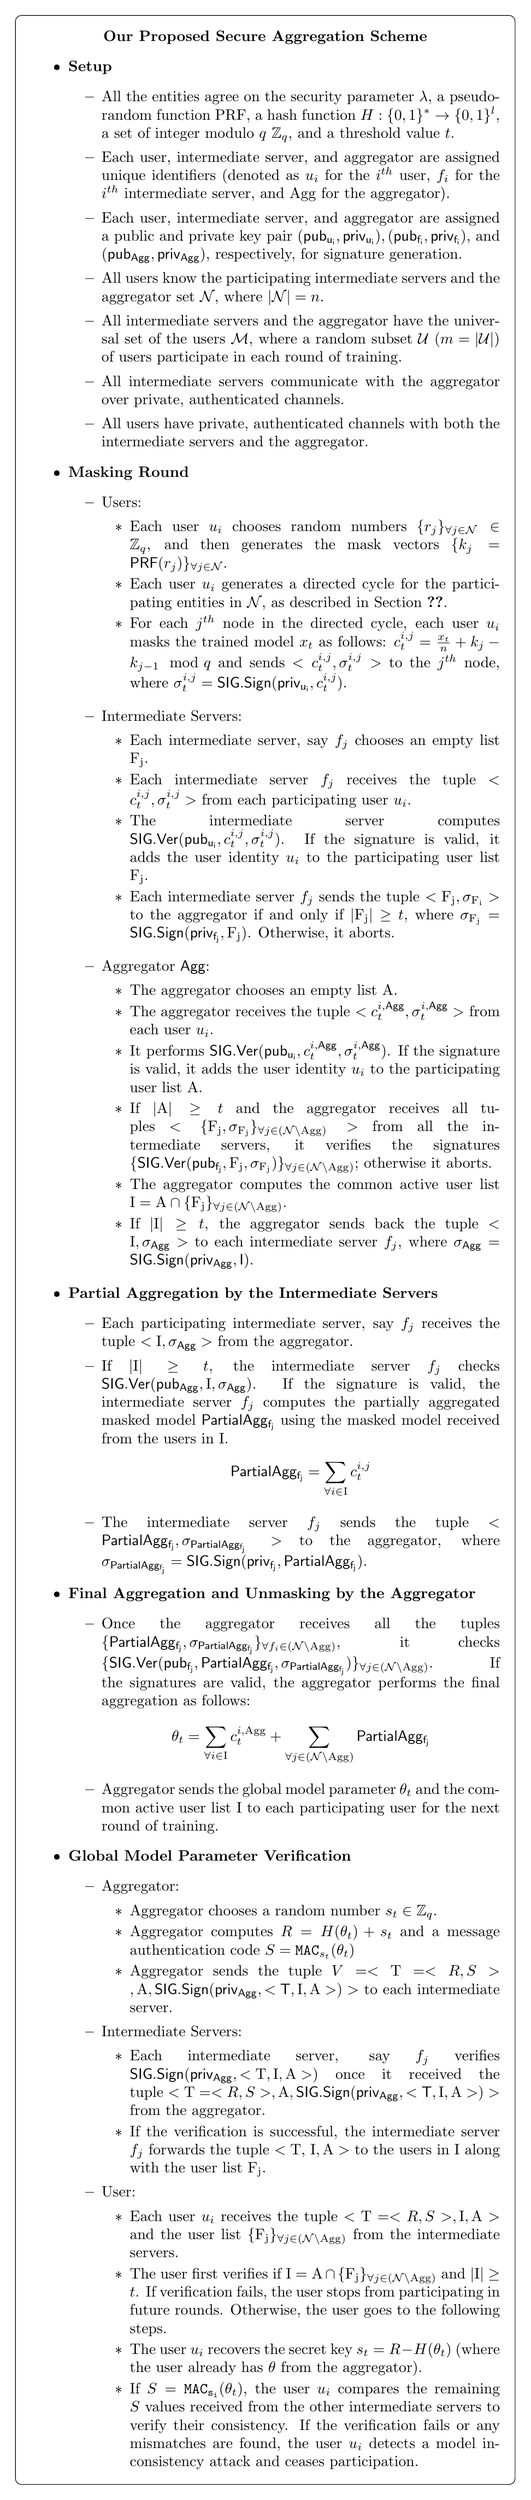
\begin{tikzpicture}[
    protocolbox/.style={draw, rectangle, rounded corners, inner sep=10pt},
    title/.style={font=\bfseries}
  ]
    \node[protocolbox] (protocol) {
      \begin{minipage}{.9\textwidth}
        \centering \textbf{Our Proposed Secure Aggregation Scheme}
        \begin{itemize}
            \item \textbf{Setup}
                \begin{itemize}
                \item All the entities agree on the security parameter $\lambda$, a pseudo-random function $\mathrm{PRF}$, a hash function $H: \{0, 1\}^*\rightarrow \{0, 1\}^l$, a set of integer modulo $q$ $\mathbb{Z}_q$, and a threshold value $t$.  
                \item Each user, intermediate server, and aggregator are assigned unique identifiers (denoted as $u_i$ for the $i^{th}$ user, $f_i$ for the $i^{th}$ intermediate server, and $\mathrm{Agg}$ for the aggregator). 
                \item Each user, intermediate server, and aggregator are assigned a public and private key pair $(\mathsf{pub_{u_i}}, \mathsf{priv_{u_i}}), (\mathsf{pub_{f_i}}, \mathsf{priv_{f_i}})$, and $(\mathsf{pub_{Agg}}, \mathsf{priv_{Agg}})$, respectively, for signature generation.
                %    \item All users are given a security parameter $\lambda$, a finite field $\mathbb{Z}_q$ with a large prime number $q$, \hl{and $t$ for minimum number of active participating users in a round.}
                \item All users know the participating intermediate servers and the aggregator set $\mathcal{N}$, where $|\mathcal{N}|= n$.
                \item All intermediate servers and the aggregator have the universal set of the users $\mathcal{M}$, where a random subset $\mathcal{U}$ ($m= |\mathcal{U}|$) of users participate in each round of training.
               \item All intermediate servers communicate with the aggregator over private, authenticated channels.
                \item All users have private, authenticated channels with both the intermediate servers and the aggregator.
               \end{itemize}
            \item \textbf{Masking Round}
               \begin{itemize}            
                \item Users:
                \begin{itemize}
                    \item Each user $u_i$ chooses random numbers $\{r_j\}_{\forall j\in \mathcal{N}}\in \mathbb{Z}_q$, and then generates the mask vectors $\{k_j= \mathsf{PRF}(r_j)\}_{\forall j\in \mathcal{N}}$.
                    \item Each user $u_i$ generates a directed cycle for the participating entities in $\mathcal{N}$, as described in Section \ref{sec:tech_intuition}.
                    \item For each $j^{th}$ node in the directed cycle, each user $u_i$ masks the trained model $x_t$ as follows: $c^{i, j}_t= \frac{x_t}{n}+ k_j- k_{j-1}\mod{q}$ and sends $<c^{i, j}_t, \sigma^{i, j}_t>$ to the $j^{th}$ node, where $\sigma^{i, j}_t= \mathsf{SIG.Sign}(\mathsf{priv_{u_i}}, c^{i, j}_t)$. 
                   % \item \textcolor{red}{Each user $u_i$ sends the masked trained model $c^{i, j}_t$ to the intermediate server or the aggregator associated with the node $j$ in the directed cycle.}
                \end{itemize}
             \end{itemize}
            %\item \textcolor{blue}{Choosing Participants ** change this heading later on}\\
            \begin{itemize}
                \item Intermediate Servers:
                \begin{itemize}
                     \item Each intermediate server, say $f_j$ chooses an empty list $\mathrm{F_j}$.
                    \item Each intermediate server $f_j$ receives the tuple $<c^{i, j}_t, \sigma^{i, j}_t>$ from each participating user $u_i$. 
                    \item The intermediate server computes $\mathsf{SIG.Ver}(\mathsf{pub_{u_i}}, c^{i, j}_t, \sigma^{i, j}_t)$. If the signature is valid, it adds the user identity $u_i$ to the participating user list $\mathrm{F_j}$. 
                    \item Each intermediate server $f_j$ sends the tuple $<\mathrm{F_j}, \sigma_{\mathrm{F_i}}>$ to the aggregator if and only if $|\mathrm{F_j}|\geq t$, where $\sigma_{\mathrm{F_j}}= \mathsf{SIG.Sign}(\mathsf{priv_{f_j}}, \mathrm{F_j})$. Otherwise, it aborts.
                \end{itemize}
            \end{itemize}
            \begin{itemize}
                \item Aggregator $\mathsf{Agg}$:
                \begin{itemize}
                    \item The aggregator chooses an empty list $\mathrm{A}$.
                   \item The aggregator receives the tuple $<c^{i, \mathsf{Agg}}_t, \sigma^{i, \mathsf{Agg}}_t>$ from each user $u_i$. 
                   \item It performs $\mathsf{SIG.Ver}(\mathsf{pub_{u_i}}, c^{i, \mathsf{Agg}}_t, \sigma^{i, \mathsf{Agg}}_t)$. If the signature is valid, it adds the user identity $u_i$ to the participating user list $\mathrm{A}$.
                   \item If $|\mathrm{A}|\geq t$ and the aggregator receives all tuples $<\{\mathrm{F_j}, \sigma_{\mathrm{F_j}}\}_{\forall j\in (\mathcal{N}\setminus \mathrm{Agg})}>$ from all the intermediate servers, it verifies the signatures $\{\mathsf{SIG.Ver}(\mathsf{pub_{f_j}}, \mathrm{F_j}, \sigma_{\mathrm{F_j}})\}_{\forall j \in (\mathcal{N}\setminus \mathrm{Agg})}$; otherwise it aborts. 
                   \item The aggregator computes the common active user list $\mathrm{I}= \mathrm{A}\cap \{\mathrm{F_j}\}_{\forall j \in (\mathcal{N}\setminus \mathrm{Agg})}$.
                   \item If $\mathrm{|I|}\geq t$, the aggregator sends back the tuple $<\mathrm{I}, \sigma_{\mathsf{Agg}}>$ to each intermediate server $f_j$, where $\sigma_{\mathsf{Agg}}= \mathsf{SIG.Sign(\mathsf{priv_{Agg}}, I)}$.
                \end{itemize}
            \end{itemize}
            \item \textbf{Partial Aggregation by the Intermediate Servers}
                \begin{itemize}
                   \item Each participating intermediate server, say $f_j$ receives the tuple $<\mathrm{I}, \sigma_{\mathsf{Agg}}>$ from the aggregator.
                   \item If $|\mathrm{I}|\geq t$, the intermediate server $f_j$ checks $\mathsf{SIG.Ver}(\mathsf{pub_{Agg}}, \mathrm{I}, \sigma_{\mathsf{Agg}})$. If the signature is valid, the intermediate server ${f_j}$ computes the partially aggregated masked model $\mathsf{PartialAgg_{f_j}}$ using the masked model received from the users in $\mathrm{I}$.
                   $$\mathsf{PartialAgg_{f_j}}= \sum_{\forall i\in \mathrm{I}}c^{i, j}_t$$ 
                   \item The intermediate server $f_j$ sends the tuple $<\mathsf{PartialAgg_{f_j}}, \sigma_{\mathsf{PartialAgg_{f_j}}}>$ to the aggregator, where $\sigma_{\mathsf{PartialAgg_{f_j}}}= \mathsf{SIG.Sign}(\mathsf{priv_{f_j}}, \mathsf{PartialAgg_{f_j}})$.
                \end{itemize}
            \item \textbf{Final Aggregation and Unmasking by the Aggregator} 
                \begin{itemize}
                   %\item Aggregator receives the tuple $<\mathsf{PartialAgg_{f_j}}, \sigma_{\mathsf{PartialAgg_{f_j}}}>$ from each intermediate server $f_j$. 
                   \item Once the aggregator receives all the tuples $\{\mathsf{PartialAgg_{f_j}}, \sigma_{\mathsf{PartialAgg_{f_j}}}\}_{\forall f_i \in (\mathcal{N}\setminus \mathrm{Agg})}$, it checks $\{\mathsf{SIG.Ver}(\mathsf{pub_{f_j}}, \mathsf{PartialAgg_{f_j}}, \sigma_{\mathsf{PartialAgg_{f_j}}})\}_{\forall j \in (\mathcal{N}\setminus \mathrm{Agg})}$. If the signatures are valid, the aggregator performs the final aggregation as follows:
                   $$\theta_t=\sum_{\forall i\in \mathrm{I}}c^{i, \mathrm{Agg}}_t+ \sum_{\forall j\in (\mathcal{N}\setminus \mathrm{Agg})}\mathsf{PartialAgg_{f_j}}$$
                   %\item Aggregator performs the final aggregation as follows: the final aggregation unmasks the aggregated global model parameter $\theta_t$.
                   %$$\theta_t= \mathsf{Partial_{Agg}}+ \sum_{1< j\leq n}\mathsf{PartialAgg_{f_j}}$$
                   \item Aggregator sends the global model parameter $\theta_t$ and the common active user list $\mathrm{I}$ to each participating user for the next round of training.
                \end{itemize}
            \item \textbf{Global Model Parameter Verification}
                \begin{itemize}
                \item Aggregator:
                \begin{itemize}
                  \item Aggregator chooses a random number $s_t\in \mathbb{Z}_q$. %and computes $s'_t= \mathrm{PRF}(s_t)$.
                  \item Aggregator computes $R= H(\theta_t)+ s_t$ and a message authentication code $S=\mathtt{MAC}_{s_t}(\theta_t)$
                  \item Aggregator sends the tuple $V= <\mathrm{T}= <R, S>, \mathrm{A}, \mathsf{SIG.Sign(\mathsf{priv_{Agg}}, <T, \mathrm{I, A}>)}>$ to each intermediate server.
                \end{itemize}
            \item Intermediate Servers:
                \begin{itemize}
                    \item Each intermediate server, say $f_j$ verifies $\mathsf{SIG.Sign(\mathsf{priv_{Agg}}, <\mathrm{T}, \mathrm{I, A}>)}$ once it received the tuple $<\mathrm{T}= <R, S>, \mathrm{A}, \mathsf{SIG.Sign(\mathsf{priv_{Agg}}, <T, \mathrm{I, A}>)}>$ from the aggregator.
                    \item If the verification is successful, the intermediate server $f_j$ forwards the tuple $<\mathrm{T}$, $\mathrm{I, A}>$ to the users in $\mathrm{I}$ along with the user list $\mathrm{F_j}$.
                \end{itemize}
                \item User:
                \begin{itemize}
                    \item Each user $u_i$ receives the tuple $<\mathrm{T}=<R, S>, \mathrm{I, A}>$ and the user list $\{\mathrm{F_j}\}_{\forall j\in (\mathcal{N}\setminus \mathrm{Agg})}$ from the intermediate servers.
                    \item The user first verifies if $\mathrm{I}= \mathrm{A}\cap \{\mathrm{F_j}\}_{\forall j \in (\mathcal{N}\setminus \mathrm{Agg})}$ and $|\mathrm{I}|\geq t$. If verification fails, the user stops from participating in future rounds. Otherwise, the user goes to the following steps.
                    \item The user $u_i$ recovers the secret key $s_t= R- H(\theta_t)$ (where the user already has $\theta$ from the aggregator). %and checks if $S= \mathtt{MAC_{s_t}}(\theta_t)$. 
                    \item If $S= \mathtt{MAC_{s_i}}(\theta_t)$, the user $u_i$ compares the remaining $S$ values received from the other intermediate servers to verify their consistency. If the verification fails or any mismatches are found, the user $u_i$ detects a model inconsistency attack and ceases participation.
                \end{itemize}
             \end{itemize}
        \end{itemize}
       
      \end{minipage}
    };  
  \end{tikzpicture}
  \caption{Detailed Description of Our Proposed Secure Aggregation Scheme}
  \label{fig:protocol-box}
  \end{scriptsize}
\end{figure*}

\section{Our Proposed Scheme}
\label{sec:our_scheme}
In this section, we provide a detailed explanation of our scheme. We first present the technical intuition behind the scheme, followed by a description of its main construction. %Next, we outline an extension that addresses the detection and prevention of model inconsistency attacks in Section \ref{sec:prevention_model_incons}.

\subsection{Technical Intuition}
\label{sec:tech_intuition}
Our protocol has three main entities: users, intermediate servers, and the aggregator, as described in Section \ref{sec:system-architecture}. Users mask their locally trained models, intermediate servers partially aggregate these masked models, and the aggregator completes the final aggregation, eventually unmasking the global model. In this section, we explain how masking and unmasking work, along with how our scheme manages user dropouts and detects model inconsistency. Let $x_u$ be the private vectors of a user $u$, and $\mathcal{U}$ be the set of participating users in a round. 
\par 
The main goal of our scheme is to compute $\sum_{\forall u \in \mathcal{U}} x_u$ in such a way that the aggregator cannot see the individual private vectors $x_u$ of any user. Our scheme can tolerate up to $m-2$ compromised users, where $m = |\mathcal{U}|$. This means that the aggregator will only get at most the aggregated vectors of the two honest users, without learning their individual private vectors. Moreover, our scheme ensures that no user learns any useful information about another user's private vector.
%Each user $u \in \mathcal{U}$ holds a private vector $x_u$ of size $n$, where each element of $x_u$ is assumed to belong to $\mathbb{Z}_q$ for some $q$. The main goal of our scheme is to compute $\sum_{\forall u \in \mathcal{U}} x_u$ in such a way that the aggregator cannot see the individual private vectors $x_u$ of any user. Our scheme can tolerate up to $m-2$ compromised users, where $m = |\mathcal{U}|$. This means that the aggregator will only get at most the aggregated vectors of the two honest users, without learning their individual private vectors. Moreover, our scheme ensures that no user learns any useful information about another user's private vector.

\paragraph*{\textbf{Masking}} 
In our system, there are $m$ participating users, $n$ intermediate servers along with the aggregator. We represent the set of intermediate servers and the aggregator as $\mathcal{N}$. Each user $u$ generates a random number $r_i$ in $\mathbb{Z}_q$ for each $i\in \mathcal{N}$. The user then uses a pseudo-random function $\mathsf{PRF}$ to generate a random vector $k_i= \mathsf{PRF}(r_i)$ for each random number $r_i$ to mask its model. The user $u$ masks its model $x_u$ using the formula:
\begin{align}
    c^i=& x_u + k_i \mod{q}.
\end{align}
 This masked model $c^i$ is then sent to the $i^{th}$ entity in $\mathcal{N}$. All other users follow the same process. After receiving all masked models from the participating users, the intermediate servers partially aggregate the masked models and send the results to the aggregator. The aggregator then combines these partially aggregated masked models with its own to produce the final aggregated masked model. 
 \par 
 We can observe that these masked models do not reveal any information about the user $u$'s private vector $x_u$ to the intermediate servers, the aggregator, or other users since the random vectors $\{k_i\}_{\forall i\in \mathcal{N}}$ are private to the user $u$ and function as one-time pads. 

 \paragraph*{\textbf{Unmasking using Key Negation Technique}} The masking process described earlier does not involve an unmasking step, meaning the aggregator only receives the combined masked models. To introduce the unmasking step, our scheme uses a similar key negation approach as in \cite{Burkhalter2020}, which is based on the aggregated homomorphic encryption method outlined in Equation \ref{eq:agg_cipher} (see Section \ref{sec:symmetricKeyHomoEncrypt}). The main goal is to use two random secret vectors to mask the models for each element in $\mathcal{N}$ so that these vectors cancel each other out during aggregation.
\par 
The concept behind our key negation mechanism is shown in Figure \ref{fig:key-neg}. Each node, labeled $c_i$, represents a masked model for the $i^{th}$ entity in $\mathcal{N}$, where $c_i = \mathsf{Enc_{(k_i- k_{i+1})}}(x_u) = x_u + \mathtt{k_i} - \mathtt{k_{i+1}} \mod{q}$. A directed arrow from node $c_i$ to node $c_{i+1}$ signifies the negation of key $k_{i+1}$ during the aggregation of masked models $c_i$ and $c_{i+1}$, as described in Equation \ref{eq:two-agg}.

% The masking process described earlier does not include an unmasking step, meaning the aggregator only receives the aggregated masked models. To incorporate the unmasking step, our scheme adopts a variation of the key negation approach proposed in \cite{Burkhalter2020}, which builds upon the aggregated homomorphic encryption method described in Equation \ref{eq:agg_cipher} (refer to Section \ref{sec:symmetricKeyHomoEncrypt}). The primary objective is to use a pair of random secret vectors to mask the models for each elements in $\mathcal{N}$ so that the vectors cancel each other out during aggregation. 
 %\par 
 %The basic concept of our key negation mechanism is illustrated in Figure \ref{fig:key-neg}. In the figure, each node, denoted as $c_i$, represents a masked model for the $i^{th}$ entity in $\mathcal{N}$, where $c_i = \mathsf{Enc_{k_i}}(x_u) = x_u + \mathtt{k_i} - \mathtt{k_{i+1}} \mod{q}$. A directed arrow from node $c_i$ to node $c_{i+1}$ represents the negation of key $k_{i+1}$ during the aggregation of the masked models $c_i$ and $c_{i+1}$, as shown in Equation \ref{eq:two-agg}.

\begin{flalign}
    \label{eq:two-agg}
    c_i+ c_{i+1}=& [x_u+ \mathtt{k_i}- \mathtt{k_{i+1}}] + [ x_u+ \mathtt{k_{i+1}}- \notag\\&\mathtt{k_{i+2}}]\mod{q}\notag\\
    =& [ x_u+ x_{u+1}+ \mathtt{k_i}- \cancel{\mathtt{k_{i+1}}}+ \cancel{\mathtt{k_{i+1}}}- \notag\\&\mathtt{k_{i+2}}] \mod{q}.
\end{flalign}
If a directed graph with a cycle, similar to the one shown in Figure \ref{fig:key-neg}, is generated from the entities in $\mathcal{N}$, aggregating all the masked models associated with the nodes will negate all the secret vectors, yielding the aggregated model. This process is illustrated in Equation \ref{eq:final-agg}.  
%\begin{scriptsize}
\begin{align}\label{eq:final-agg}
    \frac{\left(\sum_{1\leq i\leq n}c_i\right)}{n}=& n\cdot x_1+ n\cdot x_2+ \cdots+ n\cdot x_u+ \notag\\&(\cancel{k_1}-\cancel{k_2})+ (\cancel{k_2}-\cancel{k_1}+ \cdots+ \notag\\
    &(\cancel{k_{n-1}}- \cancel{k_n})+ (\cancel{k_n}-\cancel{k_1}))\notag\\
    =& \sum_{1\leq u\leq n}x_u.
\end{align}
%\end{scriptsize}

\paragraph*{\textbf{User Dropouts}} Before describing our user dropout mechanism, we briefly explain the one used in the BBGLR protocol. In the BBGLR protocol and its variants, users agree on shared secret values with each other. 
This ensures that their random masks cancel out during the aggregation process. If a user drops out, the aggregator must still be able to remove that user's masked contribution. To do this, the aggregator collects the secret shares from the remaining users to cancel out the dropped user’s contribution in the final aggregation. A similar method is also used in the Flamingo protocol \cite{Ma2023}, where the aggregator must contact a set of \emph{decryptors} to handle the dropped users' contributions. 
\par 
In contrast, our scheme does not require users to agree on shared secrets or interact with each other. Each user’s masked model is independent of the others, unlike the BBGLR protocol. Our dropout mechanism is straightforward and requires only an additional communication round between the intermediate servers and the aggregator. After the masking phase, each user sends their masked models to both the intermediate servers and the aggregator. Consequently, each intermediate server $f_i$ and the aggregator generate a user list, $\mathrm{F_i}$ and $\mathrm{A}$ respectively, based on the users from whom they received masked models. Finally, the aggregator obtains the common active user list, $\mathrm{A}$ by collecting the user lists $\mathrm{F_i}$ from all intermediate servers. This list represents the active users for that round, from whom all entities received a masked model. All the intermediate servers and the aggregator use the user list $\mathsf{I}$ to aggregate the masked models. This process ensures that dropped users are identified, and their contributions are excluded from the aggregation without compromising the global model.
%Our dropout mechanism is simple and involves only an additional round of communication between the intermediate servers and the aggregator, where the intermediate servers manage the dropout mechanism with help from the aggregator. After the masking phase, each user sends their masked models to the intermediate servers and the aggregator. As such, each intermediate server $f_i$ and the aggregator can generate a user list $\mathrm{F_i}$ and $\mathrm{A}$, respectively (those from whom they received masked models). Finally, the aggregator gets the common active user list, denoted as $\mathsf{I}$ by getting the user list $\mathrm{F_i}$ from all the intermediate servers. This list represents the active users for that round from whom all the entities received a masked model.
%Both the intermediate servers and the aggregator can then generate lists of participating users—those from whom they received masked models. The intermediate servers submit their user lists to the aggregator, which calculates the common active user list, denoted as $\mathsf{I}$, representing the active users for that round.
%\par 
%All the intermediate servers and the aggregator use this user list $\mathsf{I}$ to aggregate the masked models. 


%The aggregator sends the common active user list $\mathsf{I}$ back to the intermediate servers, which use this list to perform partial aggregation using only the masked models of the active users in the list $\mathsf{I}$. Finally, the aggregator computes the global model from the partially aggregated masked models. This extra communication round between the servers and the aggregator ensures that dropped users are identified, and their contributions are excluded from the partial and final aggregation steps.


\paragraph*{\textbf{Model Inconsistency Attack Detection}}
In \cite{Pasquini2022}, it is explained how a malicious server (or the aggregator in our case) can carry out a model inconsistency attack. In this type of attack, as we explained earlier, the server manipulates the global model to provide different versions to specific users, potentially exposing sensitive information about them. In \cite{Pasquini2022}, one of the suggested ways to prevent issues is to make sure all users get the exact same global model from the aggregator. Our scheme uses this approach too.
\par 
In our scheme, the aggregator sends the global model along with a MAC to the intermediate servers. These servers then pass the MACs to all active users listed in $\mathsf{I}$. Since each user gets the same MACs from every intermediate server, they can check for mismatches. If a user receives any different MACs, they stop participating in the training process, as this indicates a model inconsistency attack. 

%This ensures consistency, as no user can be targeted with a tampered model without detection. %However, the security of the scheme relies on proper key management for the MAC, ensuring that neither the aggregator nor any intermediary can manipulate the MAC without being detected %Please note that we haven't considered the intermediate servers to launch this attack, as we assume that at least one intermediate server will be honest all the time. 
%In our scheme, as the aggregator handles the common user list $\mathsf{I}$, a malicious aggregator could also try to launch the model inconsistency attacks. Our scheme integrates a model inconsistency detection mechanism for the users if a model inconsistency attack occurs. The core idea of the detection mechanism is to enable the users to make sure that all the users have received the correct/same global model. To do this, in our scheme the aggregator sends MACed global model to the intermediate servers. Afterwards, each intermediate server forwards the MACed global model to all the active users in the common user list $\mathsf{I}$. As the same MACed global model will be received by all the active users in $\mathsf{I}$ from the respective intermediate servers, each user will be able to verify if it receive the same global model parameter.  

\subsection{Main Scheme}
\label{sec:main-scheme}
Our scheme involves $m$ users and $n$ intermediate servers, along with an aggregator. Each user $u_i \in \mathcal{U}$ holds a private vector $x_t$ of size $n$ for the round $t$, where each element of $x_t$ belongs to $\mathbb{Z}_q$ for some $q$. Both $m$ and $n$ are polynomially bounded. The $i^{th}$ user and $j^{th}$ intermediate server are denoted as $u_i$ and $f_j$, respectively. The security of our scheme relies on the initial security parameter $\lambda$, which defines the overall strength of the scheme. Our scheme also uses a PKI, assigning each entity a private and public key pair for signing messages in the malicious model. The detailed description of our proposed secure aggregation scheme is shown in Figure \ref{fig:protocol-box}. 
\par 
The aggregator begins the protocol by sharing the initial global model with all participating users. The aggregator and the users communicate over private and authenticated channels. Each user then trains the model using their local datasets. Once trained, users mask their local models using the key negation mechanism described earlier and send the masked models to both the intermediate servers and the aggregator. This communication between users and intermediate servers also takes place over private and authenticated channels. 
\par 
The intermediate servers and aggregator collect masked models from at least $t$ users, where $t$ is the threshold required for each training round. This threshold $t$ is critical for maintaining the security of the masked models. For example, if only two users participate in a round, one user’s local model could be exposed to the other, increasing the risk of collusion. Therefore, the larger the value of $t$, the more secure the system becomes. The intermediate servers and the aggregator wait for a certain timeout period to gather enough masked models before aborting the process if an insufficient number is collected. Users are free to drop out at any time.
\par 
Once the intermediate servers receive the required number of masked models, they send their list of participating users, denoted as $\mathrm{F_i}$, to the aggregator if and only if $|\mathrm{F_i}|\geq t$. The aggregator generates a common active user list $\mathrm{I}$ from the lists received from the intermediate servers ${\mathrm{F_i}}_{\forall i\in (\mathcal{N}\setminus \mathrm{Agg})}$ and its own user list, $\mathrm{A}$. The aggregator then sends the list $\mathrm{I}$ to the intermediate servers. If $|\mathrm{I}|\geq t$, the intermediate servers partially aggregate the masked models of users in $\mathrm{I}$. Finally, the aggregator combines the partially aggregated values from the intermediate servers with the masked models from users in $\mathrm{I}$ to produce the plaintext global model ($\theta$) for the current training round.
\par 
Afterward, the aggregated global model $\theta$ is shared with all active participants for the next round of training. Simultaneously, the aggregator sends the tuple $V$ to each intermediate server. The intermediate server forwards a part of tuple $V$ to the users in $\mathrm{I}$ for verification. If the verification of the tuples is successful, the users participate in the next round; otherwise, they abort.
\par 
Figure \ref{fig:protocol-box} presents both the semi-honest and malicious model versions of the protocol. In the semi-honest model, where all entities follow the protocol honestly, the use of signatures and a PKI can be avoided.

\section{Security Analysis}
\label{sec:sec_analysis}
In this section, we present the security claims and their respective proofs for our proposed scheme discussed in Section \ref{sec:main-scheme}. %We assume that a subset $\mathcal{C}_c$ of the participating user set $\mathcal{U}$ in a round are dishonest. Similarly, a subset $\mathcal{}$. Our scheme should not reveal any information about the individual local models of the honest users when $|\mathcal{U}\setminus \mathcal{C}|> 2$. If we consider that three users are honest, the 

\subsection{Semi-Honest Model}
\label{sec:Honest-but-Curious}
In this section, we demonstrate that even if a threshold number of users, denoted as $t_c$, and intermediate servers, denoted as $t_f$, collude among themselves or with the aggregator, they cannot learn about the remaining genuine users' local weighted models. We follow a similar security model to those in \cite{Bonawitz2017} and \cite{Liu2023}. 
\par 
We consider three scenarios: first, a subset of users are dishonest and collude with adversaries or among themselves, while the intermediate servers and the aggregator remain honest. Second, a subset of intermediate servers are dishonest and can collude, while the users and the aggregator are honest. Third, a subset of users and intermediate servers, along with the aggregator, are dishonest and can collude. Our goal is to show that if fewer than $t_c$ (where $t_c>2$) and $t_f$ (where $t_f> 1$) entities are compromised, our scheme still protects the individual locally trained models of the remaining genuine users. We assume that $\mathbb{U}$ and $\mathbb{F}$ be the total number of users and intermediate servers, respectively. We also assume that $\mathcal{U}_i$ be the number of participating users in the $i^{th}$ round, and $x_{\mathbb{U}}$ is the locally trained models of the users $\mathbb{U}$.
\par 
Let $\mathsf{Real_{C}^{\mathbb{U}, t_c, \lambda}}(x_{\mathbb{U}}, \mathbb{U}_1, \mathbb{U}_2, \mathbb{U}_3)$ be a random variable representing the joint views of participants in $C$ during the real execution of our protocol. Let $\mathsf{Sim_{C}^{\mathbb{U}, t_c, \lambda}}(x_{C}, \mathbb{U}_1, \mathbb{U}_2, \mathbb{U}_3)$ be the combined views of participants in $C$ when simulating the protocol, with the inputs of honest participants selected randomly and uniformly, denoted by $x_C$. Following the aforementioned idea, the distributions of $\mathsf{Real_{C}^{\mathbb{U}, t_c, \lambda}}(x_{\mathbb{U}}, \mathbb{U}_1, \mathbb{U}_2, \mathbb{U}_3)$ and $\mathsf{Sim_{C}^{\mathbb{U}, t_c, \lambda}}(x_{C}, \mathbb{U}_1, \mathbb{U}_2, \mathbb{U}_3)$ should be indistinguishable.



%Let $\mathsf{Real_{C}^{\mathbb{U}, t_c, \lambda}}(x_{\mathbb{U}}, \mathbb{U}_1, \mathbb{U}_2, \mathbb{U}_3)$ be a random variable representing the joint views of participants in $C$ in real execution of our proposed protocol, and $\mathsf{Sim_{C}^{\mathbb{U}, t_c, \lambda}}(x_{C_c}, \mathbb{U}_1, \mathbb{U}_2, \mathbb{U}_3)$ be another combined views of participants in $C$ simulating the protocol that the inputs of honest participants are selected randomly and uniformly denoted with $x_C$. Following above-mentioned idea, the distribution of $\mathsf{Real_{C}^{\mathbb{U}, t_c, \lambda}}(x_{\mathbb{U}}, \mathbb{U}_1, \mathbb{U}_2, \mathbb{U}_3)$ and $\mathsf{Sim_{C}^{\mathbb{U}, t_c, \lambda}}(x_{C_c}, \mathbb{U}_1, \mathbb{U}_2, \mathbb{U}_3)$ should be indistinguishable.

\begin{theorem}{(Security Against Semi-Honest Users only)}\label{theorem:1}
    For all $\mathbb{U}, \mathbb{F}, \mathsf{t_c}, \lambda$ with $|C_c|< \mathsf{t_c}, x_{\mathbb{U}}, \mathbb{U}_1, \mathbb{U}_2, \mathbb{U}_3$ and $C_c$ such that $C_c\subseteq \mathbb{U}, \mathbb{U}_3\subseteq \mathbb{U}_2 \subseteq\mathbb{U}_1 \subseteq \mathbb{U}$, there exists a probabilistic-time (PPT) simulator $\mathsf{Sim_{C}^{\mathbb{U}, t_c, \lambda}}$ which output is perfectly indistinguishable from the output of $\mathsf{Real_{C}^{\mathbb{U}, t_c, \lambda}}$:
    $$\mathsf{Sim_{C}^{\mathbb{U}, t_c, \lambda}}(x_{C_c}, \mathbb{U}_1, \mathbb{U}_2, \mathbb{U}_3)\equiv \mathsf{Real_{C}^{\mathbb{U}, t_c, \lambda}}(x_\mathbb{U}, \mathbb{U}_1, \mathbb{U}_2, \mathbb{U}_3)$$
\end{theorem}
\begin{proof}\label{proof:1}
In our scheme, users randomly choose their input values (i.e., random secret keys) to mask the local model parameters, similar to a one-time pad. Each user's input values are independent of those of other users. Since the aggregator and intermediate servers are considered honest entities, the combined view of the users in $C_c$ will not reveal any useful information about the input values of users not in $C_c$. Additionally, the honest-but-curious users in $C_c$ only receive the identities of the honest users not in $C_c$. This enables the simulator $\mathsf{Sim_{C}^{\mathbb{U}, t_c, \lambda}}$ to use dummy input values for the honest users not in $C_c$ while keeping the combined views of the users in $C_c$ identical to that of $\mathsf{Real_{C}^{\mathbb{U}, t_c, \lambda}}$.


%    In our scheme, the users choose their input values (i.e., secret keys) randomly to mask the local model parameter (similar to onetime pad). Each user's input values are independent of the input values of the other users. Also, as the aggregator and the fog nodes are considered as honest entities, the combined view of the users in $C_c$ will not reveal any useful information of the input values of the users who are not in $C_c$. Further, the honest-but-curious users in $C_c$ only receive the identities of the honest users who are not in $C_c$. This enable the simulator $\mathsf{Sim_{C}^{\mathbb{U}, t_c, \lambda}}$ to use dummy input values for the honest users who are not in $C_c$ while keeping the combined views of the users in $C_c$ identical to that of $\mathsf{Real_{C}^{\mathbb{U}, t_c, \lambda}}$.

\end{proof}
\begin{theorem}{(Security Against Semi-Honest Intermediate Servers only)}\label{theorem:2}
    For all $\mathbb{U}, \mathbb{F}, \mathsf{t_f}, \lambda$ with $|C_f|\leq \mathsf{t_f}, x_{\mathbb{U}}, \mathbb{U}_1, \mathbb{U}_2, \mathbb{U}_3$ such that $C_f\subseteq \mathbb{F}$, $\mathbb{U}_3\subseteq \mathbb{U}_2 \subseteq\mathbb{U}_1 \subseteq \mathbb{U}$, there exists a probabilistic-time (PPT) simulator $\mathsf{Sim_{C}^{\mathbb{F}, t_f, \lambda}}$ which output is perfectly indistinguishable from the output of $\mathsf{Real_{C}^{\mathbb{F}, t_f, \lambda}}$:
    $$\mathsf{Sim_{C}^{\mathbb{F}, t_f, \lambda}}(x_{C_f}, \mathbb{U}_1, \mathbb{U}_2, \mathbb{U}_3)\equiv \mathsf{Real_{C}^{\mathbb{F}, t_f, \lambda}}(x_\mathbb{U}, \mathbb{U}_1, \mathbb{U}_2, \mathbb{U}_3)$$
\end{theorem}
\begin{proof}\label{proof:2}

In this proof, we consider that the intermediate servers in $C_f$ are dishonest. Since users randomly and independently choose their masking parameters (i.e., random secret keys), the intermediate servers in $C_f$ will not gain any useful information from the public values. Similarly, users send the masked local models (which are independent of each other and similar to the one-time pads) to each intermediate server separately using a secure and authenticated channel. Therefore, the joint views of the intermediate servers in $C_f$ are independent of those of the users and intermediate servers not in $C_f$. Consequently, the simulator $\mathsf{Sim_{C}^{\mathbb{U}, t_f, \lambda}}$ can use dummy input values for the intermediate servers not in $C_f$ while keeping the combined views of the intermediate servers in $C_f$ identical to those in $\mathsf{Real_{C}^{\mathbb{F}, t_f, \lambda}}$.

%   In this proof, we consider that the intermediate servers in $C_f$ are dishonest. As the users choose their masking parameters (i.e., secret keys) randomly and independently from each other, the intermediate servers in $C_f$ will not gain any useful information from the public values. Similarly, the users send the masked local models (which are independent of each other) to each intermediate server separately using a secure and authenticated channel. Hence, the joint views of the intermediate servers in $C_f$ are independent of that of the users and the intermediate servers who are not in $C_f$. Therefore, the simulator $\mathsf{Sim_{C}^{\mathbb{U}, t_f, \lambda}}$ to use dummy input values for the users and the intermediate servers who are not in $C_f$ while keeping the combined views of the intermediate servers in $C_f$ identical to that of $\mathsf{Real_{C}^{\mathbb{F}, t_f, \lambda}}$. 
        
   % As the users and the aggregator are honest, the joint views of the intermediate servers in $C_f$ are independent of that of the intermediate servers who are not in $C_f$ and also the users in $\mathbb{U}_1$, $\mathbb{U}_2$ and $\mathbb{U}_3$. The proof is similar to the Theorem \ref{theorem:1}. Hence we omit the detail discussion. 
\end{proof}
\begin{theorem}{(Security Against Semi-Honest Aggregator and Semi-Honest Intermediate Servers)}\label{theorem:3}
    For all $\mathbb{U}, \mathbb{F}, \mathsf{t_c, t_f}, \lambda$ with $|C_c|\leq \mathsf{t_c}, |C_f|\leq \mathsf{t_f}, x_{\mathbb{U}}, \mathbb{U}_1, \mathbb{U}_2, \mathbb{U}_3$ such that $C_c\subseteq \mathbb{U}, C_f\subseteq \mathbb{F}$, $\mathbb{U}_3\subseteq \mathbb{U}_2 \subseteq\mathbb{U}_1 \subseteq \mathbb{U}$, there exists a probabilistic-time (PPT) simulator $\mathsf{Sim_{C}^{\mathbb{U}, \mathbb{F}, t_c, t_f, \lambda}}$ which output is perfectly indistinguishable from the output of $\mathsf{Real_{C}^{\mathbb{U}, \mathbb{F}, t_c, t_f, \lambda}}$:
      \begin{align}
    &\mathsf{Sim_{C}^{\mathbb{U}, \mathbb{F}, t_c, t_f, \lambda}}(x_{C_c}\cup x_{C_f}, \mathbb{U}_1, \mathbb{U}_2, \mathbb{U}_3)\equiv \notag\\
    &\mathsf{Real_{C}^{\mathbb{U}, \mathbb{F}, t_c, t_f, \lambda}}(x_\mathbb{U}, \mathbb{U}_1, \mathbb{U}_2, \mathbb{U}_3) \notag
    \end{align}
\end{theorem}
\begin{proof}
    We present the detailed security proof in the Appendix \ref{proof:semihonest}. 
\end{proof}

\subsection{Malicious Model}
\label{sec:active-adversary}
In this section, we follow the standard security model as in \cite{Bonawitz2017} and \cite{Liu2023} to demonstrate that our scheme is secure against active malicious attackers. 
\par 
In this security model, we need to consider three cases. The first case is the \emph{Sybil Attack}, where the adversaries can simulate a specific honest user $u_i$ to get its inputs. Please note that our scheme is resistant to this attack, as it uses digital signatures to verify the origin of the messages. The second case involves the aggregator sending different lists of participating users in a round to the honest intermediate servers. This could lead to the disclosure of the local weighted models of the honest users. Our scheme detects this type of attack during the model parameter verification phase, where each user can verify the list of participating users in a round received from the fog servers. Any difference in the lists will indicate an attack. 
\par 
The third case involves an aggregator dishonestly dropping honest users at any round. We use the Random Oracle model to prove that our scheme is secure against any malicious dropout of honest users by adversaries. Let's consider $M_c$ as a probabilistic polynomial-time algorithm representing the \emph{next message} function of participants in $C$, which enables users in $C$ to dynamically select their inputs at any round of the protocol and the list of participating users. The Random Oracle can output the sum of a dynamically selected subset of honest clients for the simulator $\mathrm{Sim}$, which is indistinguishable from the combined view of adversaries in the real protocol execution $\mathsf{Real}(M_c)$. There are three possible scenarios for this type of active attack: first, the malicious users can collude among themselves; second, the malicious intermediate servers can collude among themselves; and finally, the malicious users and intermediate servers can collude with the aggregator. We present the following three theorems to demonstrate our security proofs.

\begin{table*}[htbp]
\centering
\caption{Running Time in Microseconds for User, Intermediate Server, and Aggregator in Different Phases Under Semi-Honest Model with a Vector Size of $50$k, $64$-bit Length, and $10$ Intermediate Servers per Round.}
\label{table:running-time-semi-honest-model}
\begin{tabular}{|p{4cm}|cc|cc|cc|cc|}
\hline
User Drop Outs & \multicolumn{2}{c|}{$0\%$} & \multicolumn{2}{c|}{$10\%$} & \multicolumn{2}{c|}{$20\%$} & \multicolumn{2}{c|}{$30\%$} \\ \hline
No. of Users & \multicolumn{1}{c|}{$500$} & $1000$ & \multicolumn{1}{c|}{$500$} & $1000$  & \multicolumn{1}{c|}{$500$} & $1000$  & \multicolumn{1}{c|}{$500$} & $1000$  \\ \hline
Masking Time at User & \multicolumn{1}{c|}{$4031$} & $4025$ & \multicolumn{1}{c|}{$3915$} &$4096$& \multicolumn{1}{c|}{$4099$} & $4085$ & \multicolumn{1}{c|}{$3921$} &  $4043$\\ \hline
Partial Aggregation Time at Intermediate Server & \multicolumn{1}{c|}{$26014.9$} & $51575.8$ & \multicolumn{1}{c|}{$23951.7$} & $46535.6$ & \multicolumn{1}{c|}{$21353$} & $43355.2$ & \multicolumn{1}{c|}{$18348.5$} & $35440.2$ \\ \hline
Final Aggregation Time at Aggregator& \multicolumn{1}{c|}{$26816$} & $52422$ & \multicolumn{1}{c|}{$24755$} & $47422$ & \multicolumn{1}{c|}{$22109$} & $44262$ & \multicolumn{1}{c|}{$19101$} & $36284$ \\ \hline
Initiation of Global Model Parameter Verification Time at Aggregator & \multicolumn{1}{c|}{$3924$} & $3936$ & \multicolumn{1}{c|}{$3938$} & $3931$ & \multicolumn{1}{c|}{$3944$} & $3930$ & \multicolumn{1}{c|}{$3881$} & $3918$ \\ \hline
Global Model Parameter Verification Time at User & \multicolumn{1}{c|}{$3748$} & $3746$ & \multicolumn{1}{c|}{$3754$} & $3764$ & \multicolumn{1}{c|}{$3757$} & $3739$ & \multicolumn{1}{c|}{$3704$} & $3749$ \\ \hline
Aggregator Total Running Time & \multicolumn{1}{c|}{$30740$} & $56358$ & \multicolumn{1}{c|}{$28693$} & $51353$ & \multicolumn{1}{c|}{$26053$} & $48192$ & \multicolumn{1}{c|}{$22982$} & $40202$ \\ \hline
Intermediate Server Total Running Time & \multicolumn{1}{c|}{$26343$} & $52218$ & \multicolumn{1}{c|}{$24254$} & $47135$ & \multicolumn{1}{c|}{$21629$} & $43908$ & \multicolumn{1}{c|}{$18590$} & $35926$ \\ \hline
User Total Running Time & \multicolumn{1}{c|}{$7779$} & $7771$ & \multicolumn{1}{c|}{$7669$} & $7860$ & \multicolumn{1}{c|}{$7853$} & $7824$ & \multicolumn{1}{c|}{$7625$} &  $7792$\\ \hline
\end{tabular}
\vspace{-.05cm}
\end{table*}

\begin{table*}[htbp]
\centering
\caption{Running Time in Microseconds for User, Intermediate Server, and Aggregator in Different Phases under the Malicious Model with a Vector Size of $50k$, 64-bit Length, and 10 Intermediate Servers per Round.}
\label{table:running-time-malicious-honest-model}
\begin{tabular}{|p{4cm}|cc|cc|cc|cc|}
\hline
User Drop Outs & \multicolumn{2}{c|}{$0\%$} & \multicolumn{2}{c|}{$10\%$} & \multicolumn{2}{c|}{$20\%$} & \multicolumn{2}{c|}{$30\%$} \\ \hline
No. of Users & \multicolumn{1}{c|}{$500$} & $1000$ & \multicolumn{1}{c|}{$500$} & $1000$  & \multicolumn{1}{c|}{$500$} & $1000$  & \multicolumn{1}{c|}{$500$} & $1000$  \\ \hline
Masking Time at User & \multicolumn{1}{c|}{$7671$} & $7702$ & \multicolumn{1}{c|}{$7654$} & $7739$ & \multicolumn{1}{c|}{$7681$} & $7721$ & \multicolumn{1}{c|}{$7679$} & $7840$ \\ \hline
Partial Aggregation Time at Intermediate Server & \multicolumn{1}{c|}{$29025$} &$55369.2$  & \multicolumn{1}{c|}{$25993$} & $52227$ & \multicolumn{1}{c|}{$23671$} & $43868$ & \multicolumn{1}{c|}{$21049$} & $38870$ \\ \hline
Final Aggregation Time at Aggregator & \multicolumn{1}{c|}{$55445$} & $82123$ & \multicolumn{1}{c|}{$52090$} & $78668$ & \multicolumn{1}{c|}{$50075$} & $70064$ & \multicolumn{1}{c|}{$47305$} & $65132$ \\ \hline
Initiation of Global Model Parameter Verification Time at the Aggregator & \multicolumn{1}{c|}{$7671$} & $7702$ & \multicolumn{1}{c|}{$7654$} & $7739$ & \multicolumn{1}{c|}{$7681$} & $7721$ & \multicolumn{1}{c|}{$7679$} & $7840$ \\ \hline
Global Model Parameter Verification Time at User & \multicolumn{1}{c|}{$3777$} & $3797$ & \multicolumn{1}{c|}{$3774$} & $3810$ & \multicolumn{1}{c|}{$3782$} & $3807$ & \multicolumn{1}{c|}{$3783$} & $3817$ \\ \hline
Aggregator Total Running Time & \multicolumn{1}{c|}{$63116$} & $89825$ & \multicolumn{1}{c|}{$59744$} & $86407$ & \multicolumn{1}{c|}{$57756$} & $77785$ & \multicolumn{1}{c|}{$54984$} & $72972$ \\ \hline
Intermediate Server Total Running Time & \multicolumn{1}{c|}{$1286470$} &$2534286$  & \multicolumn{1}{c|}{$1145840$} & $2313726$ & \multicolumn{1}{c|}{$1024000$} & $2044189$ & \multicolumn{1}{c|}{$892556$} & $1786718$  \\ \hline
User Total Running Time & \multicolumn{1}{c|}{$49112$} & $49368$ & \multicolumn{1}{c|}{$49014$} & $49678$ & \multicolumn{1}{c|}{$49220$} & $49515$ & \multicolumn{1}{c|}{$49001$} & $49498$ \\ \hline
\end{tabular}
\end{table*}


\begin{figure*}[htbp]
     \centering
     \begin{subfigure}[htbp]{0.44\textwidth}
         \centering
         \includegraphics[width=\textwidth]{image/1-IntermediateServerComTime-10IntermNodes-SemiHonest.pdf}
         \caption{Intermediate Server Average Running Time in Microseconds per Round}
         \label{fig:1-IntermediateServerComputationTimeSemiHonestModel}
     \end{subfigure}
    \hspace{.2cm}
     \begin{subfigure}[htbp]{0.44\textwidth}
         \centering
         \includegraphics[width=\textwidth]{image/1-AggregatorCompTime-SemiHonest.pdf}
         \caption{Aggregator Running Time in Microseconds per Round}
         \label{fig:1-AggregatorComputationTimeSemiHonestModel}
     \end{subfigure}
        \caption{Average Running Time of an Intermediate Server and the Aggregator with No User Dropout while Varying the Number of Users in the Semi-Honest Model per Round}
        \label{fig:1-semi-honest-ComputationTime-withoutDropout}
\end{figure*}

\begin{figure*}[htbp]
     \centering
     \begin{subfigure}[htbp]{0.44\textwidth}
         \centering
         \includegraphics[width=\textwidth]{image/1-InterServer-CompTime-Malicious-10FogNodes.pdf}
         \caption{Intermediate Server Average Running Time in Seconds per Round}
         \label{fig:1-intermediateServerComputationTimeMaliciousModel}
     \end{subfigure}
     \hspace{.2cm}
     \begin{subfigure}[htbp]{0.44\textwidth}
         \centering
         \includegraphics[width=\textwidth]{image/1-AggregatorComTime-Malicious-10FogNodes.pdf}
         \caption{Aggregator Running Time in Microseconds per Round}
         \label{fig:1-AggregatorComputationTimeMaliciousModel}
     \end{subfigure}
        \caption{Average Running Time of an Intermediate Server and the Aggregator with No User Dropout while Varying the Number of Users in a Malicious Model per Round}
        \label{fig:1-malicious-ComputationTime-withoutDropout}
\end{figure*}


\begin{figure*}[htbp]
     \centering
     \begin{subfigure}[htbp]{0.44\textwidth}
         \centering
         \includegraphics[width=\textwidth]{image/2-InterServer-ComputationTime-10FogNodes-SemiHonestModel.pdf}
         \caption{An Intermediate Server Average Running Time in Microseconds per Round}
         \label{fig:2-IntermediateServerComputationTimeSemiHonestModel}
     \end{subfigure}
     \hspace{.2cm}
     \begin{subfigure}[htbp]{0.44\textwidth}
         \centering
         \includegraphics[width=\textwidth]{image/2-Server-ComputationTime-10FogNodes-SemiHonestModel.pdf}
         \caption{Aggregator Running Time in Microseconds per Round}
         \label{fig:AggregatorComputationTimeSemiHonestModel}
     \end{subfigure}
        \caption{Average Running Time of an Intermediate Server and the Aggregator with No User Dropout while Varying the Size of Vectors in a Semi-Honest Model per Round}
        \label{fig:2-semi-honest-ComputationTime-withoutDropout}
\end{figure*}

\begin{figure*}[htbp]
     \centering
     \begin{subfigure}[htbp]{0.44\textwidth}
         \centering
         \includegraphics[width=\textwidth]{image/2-InterServer-ComputationTime-10FogNodes-MaliciousModel.pdf}
         \caption{An Intermediate Server Average Running Time in Microseconds per Round}
         \label{fig:2-intermediateServerComputationTimeMaliciousModel}
     \end{subfigure}
     %\hfill
     \hspace{.2cm}
     \begin{subfigure}[htbp]{0.43\textwidth}
         \centering
         \includegraphics[width=\textwidth]{image/2-Server-ComputationTime-10FogNodes-MaliciousModel.pdf}
         \caption{Aggregator Running Time in Microseconds per Round}
         \label{fig:2-AggregatorComputationTimeMaliciousModel}
     \end{subfigure}
        \caption{Average Running Time of an Intermediate Server and the Aggregator with No User Dropout while Varying the Size of Vectors in a Malicious Model per Round}
        \label{fig:2-malicious-ComputationTime-withoutDropout}
\end{figure*}

\begin{theorem}{(Security Against Dishonest Users only)}\label{theorem:4}
For all $\mathbb{U}, \mathbb{F}, \mathsf{t_c}, \lambda$ with $|C_c|\leq \mathsf{t_c}, x_{\mathbb{U}\setminus C_c}, \mathbb{U}$ and $C_c$ such that $C_c\subseteq \mathbb{U}$, there exists a probabilistic-time (PPT) simulator $\mathsf{Sim_{C}^{\mathbb{U}, t_c, \lambda}}$ which output is perfectly indistinguishable from the output of $\mathsf{Real_{C}^{\mathbb{U}, t_c, \lambda}}$:
$$\mathsf{Sim_{C}^{\mathbb{U}, t_c, \lambda}}(M_c, x_{\mathbb{U}\setminus C_c})\equiv \mathsf{Real_{C}^{\mathbb{U}, t_c, \lambda}}(M_c)$$
\end{theorem}
\begin{proof}
    This proof is similar to that of Theorem \ref{theorem:1}, as the users in $C_c$ gain no knowledge about $x_{\mathbb{U}\setminus C_c}$. Consequently, the simulator $\mathsf{Sim}$ can assign real inputs to the dishonest users while assigning dummy inputs to the remaining users, accurately replicating the perspectives of the users in $C_c$. Thus, the joint views of the users in $C_c$ in the simulation are indistinguishable from those in $\mathsf{Real}$.
\end{proof}


\begin{theorem}{(Security Against Dishonest Intermediate Servers only)}\label{theorem:5}
For all $\mathbb{U}, \mathbb{F}, \mathsf{t_f}, \lambda$ with $|C_f|\leq \mathsf{t_f}, x_{\mathbb{U}\setminus C_f}, \mathbb{U}$ and $C_f$ such that $C_f\subseteq \mathbb{F}$, there exists a probabilistic-time (PPT) simulator $\mathsf{Sim_{C}^{\mathbb{F}, t_f, \lambda}}$ which output is perfectly indistinguishable from the output of $\mathsf{Real_{C}^{\mathbb{F}, t_f, \lambda}}$:
$$\mathsf{Sim_{C}^{\mathbb{F}, t_f, \lambda}}(M_c, x_{\mathbb{F}\setminus C_f})\equiv \mathsf{Real_{C}^{\mathbb{F}, t_f, \lambda}}(M_c)$$
\end{theorem}
\begin{proof}
    This proof is similar to that of Theorem \ref{theorem:2}, as the intermediate servers in $C_f$ gain no knowledge about $x_{\mathbb{F}\setminus C_f}$ apart from the list of participants. Consequently, the simulator $\mathsf{Sim}$ can assign real inputs to the dishonest intermediate servers while assigning dummy inputs to the remaining intermediate servers, accurately replicating the perspectives of the intermediate servers in $C_f$. Thus, the joint views of the intermediate servers in $C_f$ in the simulation are indistinguishable from those in $\mathsf{Real}$.
\end{proof}

\begin{theorem}{(Security Against Dishonest Users, Intermediate Servers and Aggregator)}\label{theorem:6}
 For all $\mathbb{U}, \mathbb{F}, \mathsf{t_c, t_f}, \lambda$ with $|C_c|\leq \mathsf{t_c}, |C_f|\leq \mathsf{t_f}, x_{\mathbb{U}\setminus (C_c \bigcup C_f)}, \mathbb{U}$ such that $C_c\subseteq \mathbb{U}, C_f\subseteq \mathbb{F}$, $\delta_c= t_c- |C_c \cap \mathbb{U}|, \delta_f= t_f- |C_f \cap \mathbb{F}|$, there exists a probabilistic-time (PPT) simulator $\mathsf{Sim_{C}^{\mathbb{U}, t_c, t_f, \lambda}}$ which output is perfectly indistinguishable from the output of $\mathsf{Real_{C}^{\mathbb{U}, t_c, t_f, \lambda}}$:
    \begin{align*}
        &\mathsf{Sim_{C}^{\mathbb{U}, \mathbb{F}, t_c, t_f, \lambda}}(M_c, \{x_{\mathbb{U}\setminus (C_c\bigcup C_f)}\bigcup x_{\mathbb{F}\setminus C_f}\})\equiv \\
        &\mathsf{Real_{C}^{\mathbb{U}, \mathbb{F}, t_c, t_f, \lambda}}(M_c)
    \end{align*}
    where $\delta_c, \delta_f$ are the lower bound of the number of participating honest users and intermediate servers respectively.
\end{theorem}
\begin{proof}
    We present the detailed security proof in the Appendix \ref{proof:malicious}. 
\end{proof}

\section{Performance Evaluation}
\label{sec:performance_eval}
In this section, we first present a theoretical performance evaluation, covering computation and communication complexity, as well as dropout resilience, followed by the experimental results of our scheme.

\subsection{Theoretical Analysis}
\label{sec:theoritical-analysis}
We structure our theoretical analysis into two main categories: computation and communication complexity, and security and functionality. We compare our scheme with closely related works, including SecAgg \cite{Bonawitz2017}, SecAgg+ \cite{Bell2020}, TurboAgg \cite{So2021}, FastSecAgg \cite{Kadhe2020}, and EDRAgg \cite{Liu2023}.
\par 
Section \ref{sec:computation-complexity} provides a detailed analysis of the computation and communication costs for users, intermediate servers, and the main aggregator, highlighting the worst-case scenarios. While our approach introduces an intermediate server layer, which adds some additional cost, this layer contributes to improved overall performance, as we will show. Please also note that our scheme assumes a constant a fix number of intermediate servers.
\par 
In Section \ref{sec:security&functionality}, we evaluate our scheme against related works based on essential security and functionality criteria, including threat model support, resistance to model inconsistency attacks, and tolerance for user dropouts.

%We divide the theoretical analysis into two categories: computation and communication complexity analysis, and security and functionality comparison. We compare our scheme with closely related works, including SecAgg \cite{Bonawitz2017}, SecAgg+ \cite{Bell2020}, TurboAgg \cite{So2021}, FastSecAgg \cite{Kadhe2020}, and EDRAgg \cite{Liu2023}. The computation and communication complexity analysis, presented in Section \ref{sec:computation-complexity}, outlines the computation and communication costs incurred by users, intermediate servers, and the aggregator in the worst case. Unlike related schemes, our approach introduces an intermediate server layer, which adds additional cost. However, as we will demonstrate, this extra cost ultimately leads to better performance. In Section \ref{sec:security&functionality}, we compare our scheme with the related works in terms of some essential security and functionality requirements such as supported threat model, \hl{model inconsistency attack resistance}, supported user dropouts. 



%In terms of dropout resiliency, we compare the maximum tolerable dropout rates of our scheme with others. Our scheme assumes a constant, smaller number of intermediate servers compared to the number of users and input vector size. Table \ref{table:fun-com-commu-comparison} presents a comparative analysis of our scheme and related works across several dimensions, including computation and communication complexity, user dropout resilience, supported threat models for privacy, required communication rounds, setup phases in each iteration, and \hl{resilience against model inconsistency attacks.}  

%We divide the theoretical analysis into three main categories: computation complexity analysis, communication complexity analysis, and dropout resiliency. We compare our scheme with the closely related works such as SecAgg \cite{Bonawitz2017}, SecAgg+ \cite{Bell2020}, TurboAgg \cite{So2021}, FastSecAgg \cite{Kadhe2020}, and EDRAgg \cite{Liu2023}. The computation complexity analysis, which is presented in Section \ref{sec:computation-complexity}, shows the computation cost incurred at the user, intermediate servers, and the aggregator sides in the worst case. While the communication complexity analysis, which is presented in Section \ref{sec:communication-complexity}, presents the communication overhead incurred at the user, intermediate servers, and the aggregator side in the worst case. Please note that, unlike the closely related schemes, our scheme has the intermediate server layer which incurs additional cost. However, we will see in the following sections that this additional cost actually making our scheme perform better than the others. In the dropout resiliency, we show a comparison of tolerable user dropout amounts of our scheme and others. Please also note that our scheme considers the number of intermediate servers to be constant and a smaller value compared with the number of users and input vector size. 


%\hl{We consider the total number of participating intermediate servers are considered fixed (or constant), which is typically a much smaller value compared with the size of the input vector $|v|$.}
\subsubsection{Computation and Communication Complexity Analysis}\label{sec:computation-complexity}
In our scheme, each user experiences a computation complexity of $\mathcal{O}(|v|)$, primarily due to the generation of $|v|$ masking parameters for the input vector as shown in Table \ref{table:fun-com-commu-comparison}. Both the intermediate server and the aggregator have a computation complexity of $\mathcal{O}(m + |v|)$, stemming from the partial and final aggregation of masking parameters from $m$ participating users. As highlighted in Table \ref{table:fun-com-commu-comparison}, our scheme significantly reduces computation time at both the user and aggregator levels, while introducing a manageable additional $\mathcal{O}(m + |v|)$ complexity for the intermediate server. Notably, this extra complexity is well-suited to the intermediate servers, which are typically much more computationally powerful than users, further enhancing the overall efficiency of our approach.
%In our scheme, each user incurs a computation complexity of $\mathcal{O}(|v|)$, primarily due to generating $|v|$ masking parameters for the input vector. The intermediate server and the aggregator have a computation complexity of $\mathcal{O}(m + |v|)$, resulting from partial and final aggregation operations on the masking parameters received from $m$ participating users. From Table \ref{table:fun-com-commu-comparison}, we observe that our scheme reduces computation time for both users and the aggregator, although it introduces an additional $\mathcal{O}(m + |v|)$ complexity for the intermediate server. Please note that the intermediate servers are typically computationally powerful devices, unlike the users. %As such, our scheme does 
\par 
In our scheme, each user transmits its masked model parameters to the intermediate servers (with the number of intermediaries kept constant) and the aggregator, resulting in a communication complexity of $\mathcal{O}(|v|)$ for the user. Correspondingly, the communication complexity at both the intermediate server and the aggregator is $\mathcal{O}(m \cdot |v|)$. As demonstrated in Table \ref{table:fun-com-commu-comparison}, our scheme significantly reduces the communication overhead for both the user and aggregator compared to related works, largely by avoiding the use of Shamir's secret sharing technique and eliminating direct user-aggregator communication during the masking phase. Although our scheme introduces additional communication costs for the intermediate servers, these are manageable given that intermediate servers mainly communicate with the aggregator and are typically more robust in handling higher loads. This design ensures a more scalable and efficient communication process, particularly in environments with large numbers of users. Additionally, our scheme introduces a communication complexity of $\mathcal{O}(n)$ per user due to the need to receive the tuple $\big<R, S\big>$. This complexity supports our scheme's unique capability to detect model inconsistency attacks, providing a valuable enhancement in security that is not available in other approaches.

%In our scheme, each user sends its masking model parameter to each intermediate servers (as stated earlier, the number of intermediate servers is constant) and the aggregator, which constitutes $\mathcal{O}(|v|)$ communication complexity. As such, the communication complexity at the intermediate server and the aggregator are $\mathcal{O}(m\cdot |v|)$. From Table \ref{table:fun-com-commu-comparison}, we can observe that the communication overhead at the user and aggregator sides of our scheme are substantially less than the closely related works due to the avoidance of Shamir's secret sharing technique and user communication with aggregator during the setup phase respectively. However, as our scheme adds additional communication cost for the intermediate servers, which mainly communicate with the aggregator. 


\subsubsection{Security and Functionality Comparison}\label{sec:security&functionality}
Our scheme offers robust security against both semi-honest and malicious adversaries by carefully configuring system parameters, and it maintains tolerance for user dropouts of up to $m-2$ users at any time. Unlike many existing schemes such as \cite{Bonawitz2017}, its variants and \cite{Ma2023}, our approach does not require fixed participation from the start; users can join or dropout at any stage of the training process, enhancing practical applicability. Additionally, our scheme is efficient, requiring only two rounds of communication per iteration and a single setup phase, in contrast to other methods that involve a setup phase in each iteration, leading to increased overhead. Furthermore, our scheme can detect model inconsistency attacks, adding valuable security with a manageable increase in computation and communication costs.



\subsection{Experimental Result}
\label{sec:experimental-results}
We developed a prototype of our scheme and tested it on a VM with 2 vCPUs (Intel Xeon), 16GB of RAM, and Ubuntu Server 22.04. The prototype is implemented in Python (Python 3.7.11) using PyTorch 1.13.1\footnote{\url{https://pytorch.org/}}, NumPy 1.21.6\footnote{\url{https://pypi.org/project/numpy/1.21.6/}}, and PyCryptodome 3.20\footnote{\url{https://pypi.org/project/pycryptodome/}}. %\hl{Our code is available at} \url{*****??????????add-github-link*****}.
\par 
\subsubsection{Running Time Analysis Without User Dropout}
Figure \ref{fig:1-semi-honest-ComputationTime-withoutDropout} and Figure \ref{fig:2-semi-honest-ComputationTime-withoutDropout} present the running time of an intermediate server and the aggregator during a round without any user dropouts in the Semi-Honest Model, with varying numbers of users and input vector sizes, respectively. Similarly, Figure \ref{fig:1-malicious-ComputationTime-withoutDropout} and Figure \ref{fig:2-malicious-ComputationTime-withoutDropout} show the running time for the same scenario in the Malicious Model. We considered randomly generated input vectors with $64$-bit entries as the users' local gradients. In this analysis, the average running time of one intermediate server was measured, as all intermediate servers operate in parallel. The results indicate that as the number of users and input vector sizes increase, the average running time per round grows linearly, causing the total running time for both the server and intermediate servers to scale linearly with the number of users and input vector size.

\subsubsection{Running Time Analysis With User Dropout}
In the next sets of experiments, we consider user dropouts to measure the total running time of the user, intermediate server, and aggregator, along with capturing the running time of each main phase of our scheme. Table \ref{table:running-time-semi-honest-model} and Table \ref{table:running-time-malicious-honest-model} present the running times (in microseconds) per round for users, intermediate servers, and the aggregator during various phases under the semi-honest and malicious models, respectively. It compares scenarios with different percentages of user dropouts ($0\%, 10\%, 20\%, 30\%$) and varying user counts ($500$ and $1000$). For both models, the experiments used $50k$ random input vectors with $64$-bit entries and $10$ intermediate nodes.
\par 
For each scenario, the masking time at the user remains relatively stable, showing minimal variation as the percentage of user dropouts and the number of users increase, as it is independent of both. However, the partial aggregation time at the intermediate server and final aggregation time at the aggregator increase with the number of users. The running time decreases with more user dropouts due to a reduction in the number of active participants. The global model verification time at both the aggregator and user remains consistent across different scenarios, independent of user participation and dropouts. The total running times for the aggregator and intermediate server also increase with the number of users but decrease as user dropouts increase. The total running time for the user remains stable as it is unaffected by the number of participants or dropouts.

%\subsubsection{Accuracy with/without Our Scheme}
%Our scheme does not affect the FL global model accuracy. We have evaluated the accuracy by implementing our scheme in an end-to-end manner. Two widely used benchmark datasets of MNIST and CIFAR10 are considered for evaluation. Each dataset has 50,000/10,000 training/testing images. We split the training samples among \hl{xxx}\garrison{the number here.} FL clients in IID manner---note that the purpose is to show our scheme does not affect accuracy. For model architecture for MNIST is \hl{xxx}\garrison{describe the model architecture, for example, number of convolutional layers, number of fully connected layers. If the CIFAR10 uses a different model architecture, describe it separately.}

%We have set the number of FL rounds to be \hl{xx and xx} for MNIST and CIFAR10, respectively. Without our scheme, the testing accuracy of the global model on MNIST/CIFAR10 is \hl{xxx/xxx}. With our scheme enforced to guarantee strong privacy protection, the testing accuracy of the global model on MNIST/CIFAR10 is \hl{xxx/xxx}. We can see that there is no accuracy drop once our scheme is applied.
%\garrison{There is no results related to the datasets (CIFAR10 and MNIST) we tested?}


%\section{Discussion and Future Work}
%\label{sec:discussion-future-work}


\section{Conclusion}
\label{sec:conclusion}
In this paper, we introduced a lightweight secure aggregation scheme for FL that uses a key negation-based masking technique. Our approach adds an intermediate server layer, which eliminates the need for users to communicate with each other and only requires one setup phase. This significantly reduces the burden on users. Thanks to this intermediate layer, our scheme can handle user dropouts effectively, allowing users to join the training phase at any time with just one additional round of communication between the intermediate servers and the aggregator.
\par 
Additionally, we integrated a lightweight verification mechanism for model parameters to detect inconsistencies, enhancing security against malicious aggregators. We conducted a thorough formal security analysis showing that our scheme is robust against both semi-honest and malicious environments. Our comparisons with closely related works demonstrate that our scheme is better in terms of security, functionality, and both communication and computation costs. We also implemented our scheme and presented comprehensive experimental results, proving its practical usability in real-world applications.


%\section*{Acknowledgement}
%The work has been supported by the Cyber Security Research Centre Limited whose activities are partially funded by the Australian Government’s Cooperative Research Centres Program.
%\section*{Ethics Considerations}
%We confirm that we have carefully reviewed the ethical considerations mentioned in the Call for Papers (CFP), the submission guidelines, and the ethics guidelines document. Our research is centered on creating an improved privacy-preserving Federated Learning (FL) scheme, without targeting or exploiting any known vulnerabilities, ensuring that it poses no risk to existing systems. We assert that our work upholds ethical standards and fully aligns with the latest open science policies. There are no ethical concerns regarding the methods or data used in this study.

%\section*{Open Science Compliance}
%Following open science principles, we will make all code and datasets generated during this research publicly accessible upon acceptance. Additionally, we are prepared to participate in the artifact evaluation process to ensure reproducibility if necessary. This commitment allows other researchers to replicate and build upon our experiments, helping to drive progress in the field.

%\bibliographystyle{unsrt}
%	\bibliography{reference}
 \begin{thebibliography}{10}

\bibitem{Liu2022}
Z.~Liu~\emph{et al.}
\newblock Privacy-preserving aggregation in federated learning: A survey.
\newblock {\em IEEE Transactions on Big Data}, pages 1--20, 2022.

\bibitem{Antunes2022}
R.~S. Antunes, C.~Andr\'{e}~da Costa, A.~K\"{u}derle, I.~A. Yari, and B.~Eskofier.
\newblock {Federated Learning for Healthcare: Systematic Review and Architecture Proposal}.
\newblock {\em ACM Trans. Intell. Syst. Technol.}, 13(4), May 2022.

\bibitem{Niknam2020}
S.~Niknam, H.~S. Dhillon, and J.~H. Reed.
\newblock {Federated Learning for Wireless Communications: Motivation, Opportunities, and Challenges}.
\newblock {\em IEEE Communications Magazine}, 58(6):46--51, 2020.

\bibitem{Khan2021}
L.~U. Khan, W.~Saad, Z.~Han, E.~Hossain, and C.~S. Hong.
\newblock {Federated Learning for Internet of Things: Recent Advances, Taxonomy, and Open Challenges}.
\newblock {\em IEEE Communications Surveys \& Tutorials}, 23(3):1759--1799, 2021.

\bibitem{Pang2024}
Y.~Pang, Z.~Ni, and X.~Zhong.
\newblock {Federated Learning for Crowd Counting in Smart Surveillance Systems}.
\newblock {\em IEEE Internet of Things Journal}, 11(3):5200--5209, 2024.

\bibitem{Zhu2019}
L.~Zhu, Z.~Liu, and S.~Han.
\newblock {Deep Leakage from Gradients}.
\newblock In {\em Advances in Neural Information Processing Systems}, volume~32. Curran Associates, Inc., 2019.

\bibitem{Geiping2020}
J.~Geiping, H.~Bauermeister, H.~Dr\"{o}ge, and M.~Moeller.
\newblock {Inverting gradients - how easy is it to break privacy in federated learning?}
\newblock In {\em Proceedings of the 34th International Conference on Neural Information Processing Systems}, NIPS '20, 2020.

\bibitem{zhou2023ppa}
Chunyi Zhou, Yansong Gao, Anmin Fu, Kai Chen, Zhiyang Dai, Zhi Zhang, Minhui Xue, and Yuqing Zhang.
\newblock Ppa: Preference profiling attack against federated learning.
\newblock In {\em The Network and Distributed System Security Symposium (NDSS)}, 2023.

\bibitem{Jeon2024}
J.~Jeon, J.~Kim, K.~Lee, S.~Oh, and J.~Ok.
\newblock {Gradient inversion with generative image prior}.
\newblock In {\em Proceedings of the 35th International Conference on Neural Information Processing Systems}, NIPS '21, 2024.

\bibitem{Chen2024}
J.~Chen~\emph{et al.}
\newblock {When Federated Learning Meets Privacy-Preserving Computation}.
\newblock {\em ACM Comput. Surv.}, July 2024.

\bibitem{Yin2021}
X.~Yin, Y.~Zhu, and J.~Hu.
\newblock {A Comprehensive Survey of Privacy-preserving Federated Learning: A Taxonomy, Review, and Future Directions}.
\newblock {\em ACM Comput. Surv.}, 54(6), Jul 2021.

\bibitem{Bonawitz2017}
K.~Bonawitz \emph{et al.}
\newblock Practical secure aggregation for privacy-preserving machine learning.
\newblock In {\em Proceedings of the 2017 ACM SIGSAC Conference on Computer and Communications Security}, CCS '17, page 1175–1191, New York, NY, USA, 2017. Association for Computing Machinery.

\bibitem{Bell2020}
J.~H. Bell, K.~A. Bonawitz, A.~Gasc\'{o}n, T.~Lepoint, and M.~Raykova.
\newblock {Secure Single-Server Aggregation with (Poly)Logarithmic Overhead}.
\newblock In {\em Proceedings of the 2020 ACM SIGSAC Conference on Computer and Communications Security}, CCS '20, page 1253–1269, New York, NY, USA, 2020. Association for Computing Machinery.

\bibitem{Eltaras2023}
T.~Eltaras, F.~Sabry, W.~Labda, K.~Alzoubi, and Q.~Ahmedeltaras.
\newblock {Efficient Verifiable Protocol for Privacy-Preserving Aggregation in Federated Learning}.
\newblock {\em IEEE Transactions on Information Forensics and Security}, 18:2977--2990, 2023.

\bibitem{Fereidooni2021}
H.~Fereidooni \emph{et al.}
\newblock {SAFELearn: Secure Aggregation for private FEderated Learning}.
\newblock In {\em 2021 IEEE Security and Privacy Workshops (SPW)}, pages 56--62, 2021.

\bibitem{Guo2021}
X.~Guo~\emph{et al.}
\newblock Verifl: Communication-efficient and fast verifiable aggregation for federated learning.
\newblock {\em IEEE Transactions on Information Forensics and Security}, 16:1736--1751, 2021.

\bibitem{Liu2023}
Z.~Liu, J.~Guo, K.~Y. Lam, and J.~Zhao.
\newblock {Efficient Dropout-Resilient Aggregation for Privacy-Preserving Machine Learning}.
\newblock {\em IEEE Transactions on Information Forensics and Security}, 18:1839--1854, 2023.

\bibitem{Xu2020}
G.~Xu~\emph{et al.}
\newblock Verifynet: Secure and verifiable federated learning.
\newblock {\em IEEE Transactions on Information Forensics and Security}, 15:911--926, 2020.

\bibitem{Ma2023}
Y.~Ma, J.~Woods, S.~Angel, A.~Polychroniadou, and T.~Rabin.
\newblock {Flamingo: Multi-Round Single-Server Secure Aggregation with Applications to Private Federated Learning}.
\newblock In {\em 2023 IEEE Symposium on Security and Privacy (SP)}, pages 477--496, 2023.

\bibitem{Pasquini2022}
D.~Pasquini, D.~Francati, and G.~Ateniese.
\newblock Eluding secure aggregation in federated learning via model inconsistency.
\newblock In {\em Proceedings of the 2022 ACM SIGSAC Conference on Computer and Communications Security}, CCS '22, page 2429–2443, 2022.

\bibitem{Kadhe2020}
S.~Kadhe, N.~Rajaraman, O.~O. Koyluoglu, and K.~Ramchandran.
\newblock {FastSecAgg: Scalable Secure Aggregation for Privacy-Preserving Federated Learning}, 2020.

\bibitem{Wei2020}
K.~Wei~\emph{et al.}
\newblock {Federated Learning With Differential Privacy: Algorithms and Performance Analysis}.
\newblock {\em IEEE Transactions on Information Forensics and Security}, 15:3454--3469, 2020.

\bibitem{Wang2020}
Y.~Wang, Y.~Tong, and D.~Shi.
\newblock {Federated Latent Dirichlet Allocation: A Local Differential Privacy Based Framework}.
\newblock {\em Proceedings of the AAAI Conference on Artificial Intelligence}, 34(04):6283--6290, Apr. 2020.

\bibitem{Zhou2022}
H.~Zhou~\emph{et al.}
\newblock Pflf: Privacy-preserving federated learning framework for edge computing.
\newblock {\em {IEEE Transactions on Information Forensics and Security}}, 17:1905--1918, 2022.

\bibitem{Chan2012}
T.~H.~H. Chan, E.~Shi, and D.~Song.
\newblock "privacy-preserving stream aggregation with fault tolerance".
\newblock In {\em Financial Cryptography and Data Security}, pages 200--214, 2012.

\bibitem{Phong2018}
L.~T. Phong~\emph{et al.}
\newblock {Privacy-Preserving Deep Learning via Additively Homomorphic Encryption}.
\newblock {\em IEEE Transactions on Information Forensics and Security}, 13(5):1333--1345, 2018.

\bibitem{Ma2022}
Z.~Ma~\emph{et al.}
\newblock {ShieldFL: Mitigating Model Poisoning Attacks in Privacy-Preserving Federated Learning}.
\newblock {\em IEEE Transactions on Information Forensics and Security}, 17:1639--1654, 2022.

\bibitem{Sav2021}
S.~Sav \emph{et al.}
\newblock {POSEIDON: Privacy-Preserving Federated Neural Network Learning}.
\newblock In {\em NDSS}, 2021.

\bibitem{Zhang2020Usenix}
C.~Zhang~\emph{et al.}
\newblock {BatchCrypt: efficient homomorphic encryption for cross-silo federated learning}.
\newblock In {\em Proceedings of the 2020 USENIX Conference on Usenix Annual Technical Conference}, USENIX ATC'20, 2020.

\bibitem{So2021}
J.~So, B.~Güler, and A.~S. Avestimehr.
\newblock Turbo-aggregate: Breaking the quadratic aggregation barrier in secure federated learning.
\newblock {\em IEEE Journal on Selected Areas in Information Theory}, 2(1):479--489, 2021.

\bibitem{So2022ML}
J.~So~\emph{et al.}
\newblock {LightSecAgg: a Lightweight and Versatile Design for Secure Aggregation in Federated Learning}.
\newblock In {\em Proceedings of Machine Learning and Systems}, volume~4, pages 694--720, 2022.

\bibitem{Liu2024}
Z.~Liu \emph{et al.}
\newblock {Dynamic User Clustering for Efficient and Privacy-Preserving Federated Learning}.
\newblock {\em IEEE Transactions on Dependable and Secure Computing}, (01):1--12, Jan. 2024.

\bibitem{Fu2024}
X.~Fu~\emph{et al.}
\newblock {Blockchain-Based Efficiently Privacy-Preserving Federated Learning Framework Using Shamir Secret Sharing}.
\newblock {\em IEEE Transactions on Consumer Electronics}, pages 1--1, 2024.

\bibitem{Wang2023}
Y.~Wang, A.~Zhang, S.~Wu, and S.~Yu.
\newblock {VOSA: Verifiable and Oblivious Secure Aggregation for Privacy-Preserving Federated Learning}.
\newblock {\em IEEE Transactions on Dependable and Secure Computing}, 20(5):3601--3616, 2023.

\bibitem{Yang2023}
S.~Yang, Y.~Chen, Z.~Yang, B.~Li, and H.~Liu.
\newblock {Fast Secure Aggregation With High Dropout Resilience for Federated Learning}.
\newblock {\em IEEE Transactions on Green Communications and Networking}, 7(3):1501--1514, 2023.

\bibitem{Fazli2023}
H.~Fazli~Khojir, D.~Alhadidi, S.~Rouhani, and N.~Mohammed.
\newblock {FedShare: Secure Aggregation based on Additive Secret Sharing in Federated Learning}.
\newblock In {\em Proceedings of the 27th International Database Engineered Applications Symposium}, IDEAS '23, page 25–33, New York, NY, USA, 2023. Association for Computing Machinery.

\bibitem{Burkhalter2020}
L.~Burkhalter, A.~Hithnawi, A.~Viand, H.~Shafagh, and S.~Ratnasamy.
\newblock {TimeCrypt: encrypted data stream processing at scale with cryptographic access control}.
\newblock In {\em Proceedings of the 17th Usenix Conference on Networked Systems Design and Implementation}, USENIX NSDI'20, page 835–850. USENIX Association, 2020.

\bibitem{Castelluccia2009}
C.~Castelluccia, A.~C-F. Chan, E.~Mykletun, and G.~Tsudik.
\newblock {Efficient and provably secure aggregation of encrypted data in wireless sensor networks}.
\newblock {\em ACM Trans. Sen. Netw.}, 5(3), Jun 2009.

\end{thebibliography}

\appendices

\section{Security Proof Against Semi-Honest Aggregators and Intermediate Servers}\label{proof:semihonest}
\begin{proof}
    In this proof, we use a standard hybrid argument, which consists of a sequence of hybrid distributions, to construct the simulator $\mathsf{Sim}$ by the subsequent modifications to the random variable $\mathsf{Real}$. The goal is to prove that two subsequent hybrids are computationally indistinguishable to ensure that the distribution of simulator $\mathsf{Sim}$ as a whole is also identical to the real execution $\mathsf{Real}$.
    
    \paragraph*{$\mathsf{Hyb_0}$} In this hybrid, the distribution of the joint views of $C_c$ and $C_f$ is exactly the same as that of $\mathsf{Real}$.

    \paragraph*{$\mathsf{Hyb_1}$} In this hybrid, the simulator $\mathsf{Sim}$ chooses random numbers in $\mathbb{Z}_q$ using a pseudo-random function $\mathrm{PRF}$ as the trained model for the users in $(\mathbb{U}_1\setminus C_c)$. Based on the security of the pseudo-random function, the joint views of the users in $C_c$ is identical to that of $\mathsf{Real}$. Hence, this hybrid is indistinguishable from the previous one. 
    
    \paragraph*{$\mathsf{Hyb_2}$} In this hybrid, similar to the previous one, but for each user $i$ in $(\mathbb{U}_1\setminus C_c)$, the simulator $\mathsf{Sim}$ generates separate one-time-pads to mask $r_i$ for each intermediate server in $(\mathbb{F}\setminus C_f)$ including the aggregator. Based on the security of the one-time-pad, the joint views of the users in $C_c$ and intermediate servers in $C_f$ is identical to that of $\mathsf{Real}$. Hence, this hybrid is indistinguishable from the previous one.
   
    %chooses random numbers in $\mathbb{Z}_q$ using a pseudo-random function $\mathcal{PRF}$ as the trained model for users in $(\mathbb{U}_1\setminus C_c)$ and the intermediate servers in $(\mathbb{F}\setminus C_f)$. Based on the security of the pseudo-random function, the joint views of the users in $C_f$ is identical to that of $\mathsf{Real}$. Hence, this hybrid is indistinguishable from the previous one.
    
    \paragraph*{$\mathsf{Hyb_3}$} In this hybrid, for each user $i$ in $(\mathbb{U}_1\setminus C_c)$, the simulator $\mathsf{Sim}$ chooses two random secrets $(k_j, k_{j-1})\in \mathbb{Z}_q$ to mask $r_i$ as $r_i+ k_j- k_{j-1}$ for each intermediate server $j$ in $(\mathbb{F}\setminus C_f)$ including the aggregator. Based on the semantic security (IND-CPA) of the symmetric homomorphic encryption scheme (described in Section \ref{sec:symmetricKeyHomoEncrypt}), the joint views of the users in $C_c$ and intermediate servers in $C_f$ is identical to that of $\mathsf{Real}$. Hence, this hybrid is indistinguishable from the previous one.
     
   % \hl{$\mathsf{Sim}$ chooses random values, using a pseudorandom function $\mathcal{PRF}$, as the masking parameter for the users in $(\mathbb{U}_1\setminus C_c)$ instead of the proper masking values to mask the local trained model for the entities in $\mathbb{F}$ and the aggregator. For instance, for each party $i$ in $\mathbb{F}$ including the aggregator, the $\mathsf{Sim}$ chooses a random value, say $r_i$ instead of the proper masking secrets $(k_i- k_{i-1})$ as the masking value. Based on the security of the pseudorandom function, the joint views of the users in $C_c$ is identical to that of $\mathsf{Real}$. Hence, this hybrid is indistinguishable from the previous one. }

    \paragraph*{$\mathsf{Hyb_4}$} This hybrid is similar to the previous one. The only difference is that the simulator $\mathsf{Sim}$ replaces the random masked $r_i$ for each users in $(\mathbb{U}_1\setminus C_c)$ with $x_i$ subject to 
    \begin{align}\label{eq:mask}
        \sum_{i\in \mathbb{U}_1\setminus C_c}r_i=& \sum_{\mathbb{U}_1\setminus C_c}x_i
    \end{align}
    As we can observe the distribution of the masking values generated based on the symmetric homomorphic encryption scheme for masking $r_i$ and $x_i$ is identical subject to the Eq. \ref{eq:mask}.
  
  %  proper masking parameters to the intermediate servers in $\mathbb{F}\setminus C_f$ for the users in $\mathbb{U}_1\setminus C_c$ and random values for the users in $C_c$ to the intermediate servers in $C_f$. As the symmetric homomorphic encryption scheme is semantically secure (IND-CPA), the combined views of the users in $C_c$ and intermediate servers in $C_f$ including the aggregator will not reveal any useful information on the actual trained model and their masking values. Hence, this hybrid is indistinguishable from the previous one.}
    
    
 %   ******* Sim sends random values for the users in $(\mathbb{U}_1\setminus C_c)$ and \hl{proper values} for the other users to intermediate servers in $C_f$, including the aggregator. Based on the IND-CPA security of the symmetric key additive holomorphic encryption scheme, the combined views of $C_f$ including the aggregator is identical to the $\mathsf{Real}$. Hence, this hybrid is indistinguishable from the previous one. **********  
   % \paragraph*{$\mathsf{Hyb_3}$}
   \par 
   Therefore, the last hybrid shows that we can define a simulator $\mathsf{Sim}$ which is computationally indistinguishable from that of the real execution of $\mathsf{Real}$ from the combined views of the honest-but-curious entities. Hence, it completes the proof. 
\end{proof}

\section{Security Proof Against Dishonest Users, Intermediate Servers and Aggregator}\label{proof:malicious}
\begin{proof}
    We use the standard hybrid argument to carry out the security proof of this theorem. Similar to the Theorem \ref{theorem:3}, we construct a simulator $\mathsf{Sim}$ by the subsequent modifications to the random variable $\mathsf{Real}$. Our goal is to prove that two subsequent hybrids are computationally indistinguishable to ensure that the distribution of simulator $\mathsf{Sim}$ as a whole is also identical to the real execution $\mathsf{Real}$.
    
    \paragraph*{$\mathsf{Hyb_0}$} In this hybrid, the distribution of the joint view of $M_c$ of $\mathsf{Sim}$ is the same as that of $\mathsf{Real}$.

   \paragraph*{$\mathsf{Hyb_1}$} In this hybrid, the simulator $\mathsf{Sim}$ replaces the masking values of the locally trained models with randomly generated numbers of appropriate length. Based on the security of the pseudo-random function, the joint views of the users in $M_c$ are identical to those of $\mathsf{Real}$. Hence, this hybrid is indistinguishable from the previous one.
    
    \paragraph*{$\mathsf{Hyb_2}$} In this hybrid scenario, the simulator $\mathsf{Sim}$ replaces the masked locally trained model $x_i$ of each honest user $u_i$ with a randomly generated number, while it replaces it with $0$ for the adversaries. Based on the security of the pseudo-random function, the joint views of the users in $M_c$ are identical to those of $\mathsf{Real}$. Hence, this hybrid is indistinguishable from the previous one.
  
    \paragraph*{$\mathsf{Hyb_4}$} In this hybrid, the simulator $\mathsf{Sim}$ uses the symmetric homomorphic encryption with key negation method, as described in Section \ref{sec:symmetricKeyHomoEncrypt}, to replace each mask of the locally trained model for the intermediate servers in the $\mathbb{F}'$. Based on the semantic security (IND-CPA) of the symmetric homomorphic encryption scheme, the joint views of the users in $M_c$ are identical to those of $\mathsf{Real}$. Hence, this hybrid is indistinguishable from the previous one. 

    %\paragraph*{$\mathsf{Hyb_5}$} Similar to the previous one, in this hybrid but for each user $i$ in $(\mathbb{U}\setminus C_c)$, the simulator $\mathsf{Sim}$ generates separate one-time-pads to mask $r_i$ for each intermediate server in $(\mathbb{F}\setminus C_f)$ including the Aggregator. Based on the security of the one-time-pad, the joint views of the users in $M_c$ are identical to that of $\mathsf{Real}$. Hence, this hybrid is indistinguishable from the previous one.
    
    \paragraph*{$\mathsf{Hyb_5}$} In this hybrid, the $\mathsf{SIM}$ aborts if $M_c$ provides with incorrect signatures $\sigma^{i, j}_t$ (or $\sigma^{i, \mathsf{Agg}}_t$) for each user $u_i$ in $(\mathbb{U} \setminus C_c)$. This hybrid is indistinguishable from the previous one based on the security assumption of the signature mechanism.

    \paragraph*{$\mathsf{Hyb_6}$} In this hybrid, the simulator $\mathsf{SIM}$ fetches $\mathrm{I}$ list of users from the aggregator and aborts if list has any invalid user. This hybrid is identical to the previous one. 
    
    \paragraph*{$\mathsf{Hyb_7}$} In this hybrid, the simulator $\mathsf{SIM}$ queries to the Random Oracle $\mathcal{O}$ for the values $w_i$ for the set $(\mathrm{I}\setminus C_c)$ with respect to $\sum_{u_i\in \mathcal{Q}\setminus C_c} w_i= \sum_{u_i\in \mathcal{Q}\setminus C_c}x_i$ instead of receiving the inputs of the honest users and masks it with a random number. For the adversaries, the $\mathsf{Sim}$ chooses random numbers (masks are set to be $0$ here). The Random Oracle $\mathcal{O}$ will not abort and does not modify the joint view of $M_c$ if at least more than $2$ participants are honest due to the properties of the random oracle and pseudo-random function. Thus, this hybrid is indistinguishable from the previous one.

    \paragraph*{$\mathsf{Hyb_8}$} In this hybrid, the $\mathsf{Sim}$ aborts if $M_c$ provides with incorrect signatures $\sigma^{\mathrm{F}}$ for each intermediate server $f_i$ in $(\mathbb{F} \setminus C_f)$. This hybrid is indistinguishable from the previous one based on the security assumption of the signature mechanism.

    \paragraph*{$\mathsf{Hyb_9}$} In this hybrid, the simulator $\mathsf{SIM}$ again queries to the Random Oracle $\mathcal{O}$ for the values $\{w^j_i\}_{\forall j\in \mathbb{F}\setminus C_f}$ for the set $(\mathrm{I}\setminus C_c)$ with respect to $\sum_{u_i\in \mathcal{Q}\setminus C_c} w'_i= \sum_{u_i\in \mathcal{Q}\setminus C_c}x'_i$ instead of receiving the inputs of the honest users and honest intermediate servers. The Random Oracle $\mathcal{O}$ will not abort and does not modify the joint views of $M_c$ if at least more than $2$ users are honest and $1$ intermediate server is honest. Thus, this hybrid is indistinguishable from the previous one.
\par 
It can be observed from the last hybrid that the adversary's view remains unaffected which proves the indistinguishable property between the different hybrids. Furthermore, this hybrid does not take input from honest parties. This completes the proof.
\end{proof}


\end{document}
